\documentclass[conference]{IEEEtran}
\IEEEoverridecommandlockouts

\usepackage{cite}
\usepackage{amsmath,amssymb,amsfonts}
\usepackage{mathtools}
\usepackage{algorithmic}
\usepackage{graphicx}
\usepackage{textcomp}
\usepackage{xcolor}
\usepackage{textcomp}
\usepackage{float}
\usepackage{array}
\usepackage{siunitx}
\usepackage{tabularx}
\usepackage{listings}
\usepackage{accents}
\usepackage{nicematrix,tikz}
\usepackage{setspace}
\usepackage[colorlinks=false]{hyperref}
\def\BibTeX{{\rm B\kern-.05em{\sc i\kern-.025em b}\kern-.08em
    T\kern-.1667em\lower.7ex\hbox{E}\kern-.125emX}}

\setlength{\parindent}{0pt}

% Define the custom column type Y
\newcolumntype{Y}{>{\centering\arraybackslash} m{1.1cm}}

\definecolor{codeblue}{rgb}{0.2,0.2,0.6}
\definecolor{codegreen}{rgb}{0.133,0.545,0.133}
\definecolor{codegray}{rgb}{0.5,0.5,0.5}
\definecolor{codepurple}{rgb}{0.58,0,0.82}
\definecolor{backcolour}{rgb}{0.95,0.95,0.92}

\lstdefinestyle{mystyle}{
    backgroundcolor=\color{backcolour},
    commentstyle=\color{codegreen},
    keywordstyle=\color{codeblue},
    numberstyle=\tiny\color{codegray},
    stringstyle=\color{codepurple},
    basicstyle=\ttfamily\scriptsize,
    breakatwhitespace=false,
    breaklines=true,
    captionpos=b,
    keepspaces=true,
    numbers=none,
    numbersep=5pt,
    showspaces=false,
    showstringspaces=false,
    showtabs=false,
    tabsize=2
}
\lstset{style=mystyle}

\title{Robotics and Mechatronics\\
{\LARGE Homework Three}
}

\author{\IEEEauthorblockN{Mohammad Montazeri}
    \IEEEauthorblockA{\textit{School of Mechanical Engineering} \\
        \textit{College of Engineering, University of Tehran}\\
        Tehran, Iran; 810699269 \\
        mohammadmontazeri@ut.ac.ir}
}

\begin{document}
\maketitle

\begin{abstract}
    In this homework we mainly explore the vast field of robotics regarding robot Jacobians and Trajectories. These mathematical constructs play a crucial role in controlling robotic arms for precise movements. Our report covers the essentials of these two matters, including subjects like Jacobians, singularity, static analysis, and trajectory generation using MATLAB.
\end{abstract}

\begin{IEEEkeywords}
    Jacobian, trajectory, singularity, velocity, acceleration, interpolation, end-effector
\end{IEEEkeywords}

\section{Introduction}
In robotics, the Jacobian matrix bridges joint velocities (how fast each joint moves) to the velocity of the end effector (the robotic arm’s tip). It helps us understand how changes in joint motion affect the overall movement of the arm. Jacobians find applications in controlling robotic arms during tasks like painting or precise movements. For instance, if the servo motors rotate at certain velocities, the Jacobian helps calculate how fast the end effector moves in both linear (x, y, z) and angular (roll, pitch, yaw) directions. Trajectory planning involves finding a time series of successive joint angles or end-effector positions that guide a robot from its starting configuration to a desired goal. It's like plotting the robot's path through space to achieve specific tasks, such as picking up an object and placing it on a shelf. As we delve into this fascinating realm, we'll explore how Jacobians enable precise control and discuss the importance, applications, methods and challenges of trajectory planning where motion becomes ambiguous.

\section{Problem 1: Wrist Robot Jacobian}
\begin{figure}[htbp]
    \centerline{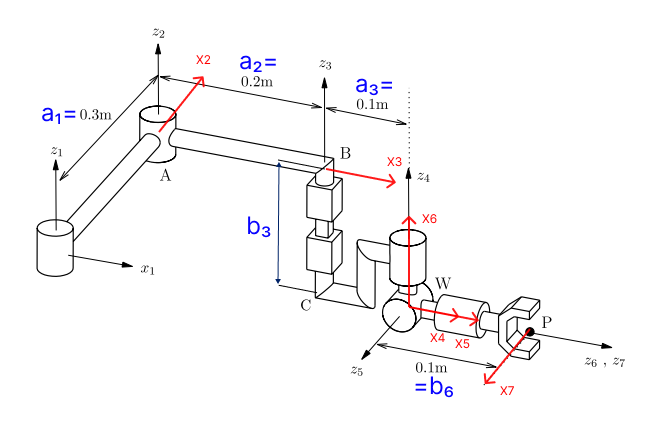
\includegraphics[width=0.4\textwidth]{figures/prob1.png}}
    \caption{Schematic view of 6-DOF robot with its D-H vectors}
    \label{fig:prob1}
\end{figure}

The velocity of end-effector, also known as its \textbf{\textit{twist}}, can be found from equation below:

\begin{align}
    \vec{t} = \begin{bmatrix}
                  \vec{\omega} \\
                  \dot{\vec{P}}
              \end{bmatrix} = \undertilde{J} \dot{\vec{\theta}} \label{eq:twist}
\end{align}

Where,
\begin{itemize}
    \item $\vec{t}$ is the twist of end-effector,
    \item $\vec{\omega}$ is the angular velocity of end-effector,
    \item $\dot{\vec{P}}$ is the linear velocity of end-effector,
    \item $\undertilde{J}$ is the Jacobian matrix,
    \item $\dot{\vec{\theta}}$ is the joints' velocity.
\end{itemize}

Since the third joint is a prismatic one in this robot, to find its Jacobian at the current configuration, we use:
\begin{align}
    \undertilde{\mathcal{J}} = \begin{bmatrix}
                                   \vec{e_1}                  & \vec{e_2}                  & \vec{O}   & \vec{e_4}                  & \vec{e_5}                  & \vec{e_6}                  \\
                                   \vec{e_1} \times \vec{r_1} & \vec{e_2} \times \vec{r_2} & \vec{e_3} & \vec{e_4} \times \vec{r_4} & \vec{e_5} \times \vec{r_5} & \vec{e_6} \times \vec{r_6} \\
                               \end{bmatrix}
\end{align}

Where, in this problem, using the fixed coordinate origin of \((x_1, y_1, z_1)\) in Figure~\ref{fig:prob1} we have:
\begin{align*}
    \vec{e_1} = \vec{e_2} = \vec{e_3} =
    \vec{e_4} = \begin{bmatrix}
                    0 \\
                    0 \\
                    1
                \end{bmatrix} \hspace{15px}
    \vec{e_5} = \begin{bmatrix}
                    0  \\
                    -1 \\
                    0
                \end{bmatrix} \hspace{15px}
    \vec{e_6} = \begin{bmatrix}
                    1 \\
                    0 \\
                    0
                \end{bmatrix}
\end{align*}

\begin{align*}
    \vec{r_1} = \begin{bmatrix}
                    0.4 \\
                    0.3 \\
                    -b
                \end{bmatrix} \hspace{4px}
    \vec{r_2} = \begin{bmatrix}
                    0.4 \\
                    0   \\
                    -b
                \end{bmatrix} \hspace{4px}
    \vec{r_3} = \begin{bmatrix}
                    0.2 \\
                    0   \\
                    -b
                \end{bmatrix} \hspace{4px}
    \vec{r_4} = \vec{r_5} = \vec{r_6} = \begin{bmatrix}
                                            0.1 \\
                                            0   \\
                                            0
                                        \end{bmatrix}
\end{align*}

So, by doing the math, the Jacobian is computed as:
\begin{align*}
    \undertilde{\mathcal{J}} = \begin{bmatrix}
                                   0    & 0   & 0 & 0   & 0   & 1 \\
                                   0    & 0   & 0 & 0   & -1  & 0 \\
                                   1    & 1   & 0 & 1   & 0   & 0 \\
                                   -0.3 & 0   & 0 & 0   & 0   & 0 \\
                                   0.4  & 0.4 & 0 & 0.1 & 0   & 0 \\
                                   0    & 0   & 1 & 0   & 0.1 & 0 \\
                               \end{bmatrix}
\end{align*}
Now, having the given joint space velocities and the obtained Jacobian, we can find the end-effector velocity by equation \ref{eq:twist}.

\begin{align*}
    \vec{t} = \begin{bmatrix}
                  \vec{\omega} \\
                  \dot{\vec{P}}
              \end{bmatrix} = \begin{bmatrix}
                                  0    & 0   & 0 & 0   & 0   & 1 \\
                                  0    & 0   & 0 & 0   & -1  & 0 \\
                                  1    & 1   & 0 & 1   & 0   & 0 \\
                                  -0.3 & 0   & 0 & 0   & 0   & 0 \\
                                  0.4  & 0.4 & 0 & 0.1 & 0   & 0 \\
                                  0    & 0   & 1 & 0   & 0.1 & 0 \\
                              \end{bmatrix} \begin{bmatrix}
                                                1 \\
                                                1 \\
                                                1 \\
                                                1 \\
                                                1 \\
                                                1 \\
                                            \end{bmatrix} = \begin{bmatrix}
                                                                1    \\
                                                                -1   \\
                                                                3    \\
                                                                -0.3 \\
                                                                0.9  \\
                                                                1.1
                                                            \end{bmatrix}
\end{align*}

This means point \textit{P} has an angular velocity of $\omega = \left[1, -1, 3\right]$ rad/s and a linear velocity of $v = \left[-0.3, 0.9, 1.1\right]$ m/s, with respect to fixed coordinate system of \((x_1, y_1, z_1)\).

\section{Problem 2: Jacobian and Singularity}
The D-H parameters of this robot were obtained from the configurations marked up in Figure~\ref{fig:prob2} which was first sketched in the previous homework. The \(Q_i\) and \(\vec{a_i}\) parameters were also derived which will be used here to form the general Jacobian matrix. Here's the previous results:

\begin{figure}[htbp]
    \centerline{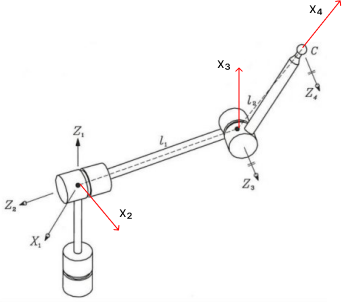
\includegraphics[width=0.4\textwidth]{figures/prob2.png}}
    \caption{Schematic view of robot marked up with D-H vectors}
    \label{fig:prob2}
\end{figure}

\begin{table}[htbp]
    \caption{The D-H parameters of 3-DOF robot}
    \def\arraystretch{1.75}
    \begin{center}
        \begin{tabular}{|Y|Y|Y|Y|Y|}
            \hline
            $i$ & $a_i$ & $b_i$  & $\alpha_i$ & $\theta_i$ \\
            \hline
            1   & 0     & 0      & $\pi / 2$  & $\theta_1$ \\
            \hline
            2   & 0     & $-l_1$ & $\pi / 2$  & $\theta_2$ \\
            \hline
            3   & $l_2$ & 0      & 0          & $\theta_3$ \\
            \hline
        \end{tabular}
    \end{center}
\end{table}

\begin{small}
    \begin{align*}
         & \left[Q_1\right] = \begin{bmatrix}
                                  \cos \theta_1 & 0 & \sin \theta_1   \\
                                  \sin \theta_1 & 0 & - \cos \theta_1 \\
                                  0             & 1 & 0
                              \end{bmatrix} & \vec{\mathbf{a_1}} =
        \begin{bmatrix}
            0 \\
            0 \\
            0
        \end{bmatrix}                                             \\
         & \left[Q_2\right] = \begin{bmatrix}
                                  \cos \theta_2 & 0 & \sin \theta_2   \\
                                  \sin \theta_2 & 0 & - \cos \theta_2 \\
                                  0             & 1 & 0
                              \end{bmatrix} & \vec{\mathbf{a_2}} =
        \begin{bmatrix}
            0 \\
            0 \\
            -l_1
        \end{bmatrix}                                             \\
         & \left[Q_3\right] = \begin{bmatrix}
                                  \cos \theta_3 & - \sin \theta_3 & 0 \\
                                  \sin \theta_3 & \cos \theta_3   & 0 \\
                                  0             & 0               & 1
                              \end{bmatrix} & \vec{\mathbf{a_3}} =
        \begin{bmatrix}
            l_2 \cos \theta_3 \\
            l_2 \sin \theta_3 \\
            0
        \end{bmatrix}
    \end{align*}
\end{small}

% \begin{small}
%     \begin{align*}
%          & \left[Q_1\right] = \begin{bmatrix}
%                                   \cos \theta_1 & 0 & \sin \theta_1   \\
%                                   \sin \theta_1 & 0 & - \cos \theta_1 \\
%                                   0             & 1 & 0
%                               \end{bmatrix} \quad
%         \left[Q_2\right] = \begin{bmatrix}
%                                \cos \theta_2 & 0 & \sin \theta_2   \\
%                                \sin \theta_2 & 0 & - \cos \theta_2 \\
%                                0             & 1 & 0
%                            \end{bmatrix}    \\
%          & \left[Q_3\right] = \begin{bmatrix}
%                                   \cos \theta_3 & - \sin \theta_3 & 0 \\
%                                   \sin \theta_3 & \cos \theta_3   & 0 \\
%                                   0             & 0               & 1
%                               \end{bmatrix} \\
%         % -------------------------
%          &                                        &               \\
%         % -------------------------
%          & \vec{\mathbf{a_1}} =
%         \begin{bmatrix}
%             0 \\
%             0 \\
%             0
%         \end{bmatrix} \quad\quad\quad
%         \vec{\mathbf{a_2}} =
%         \begin{bmatrix}
%             0 \\
%             0 \\
%             -l_1
%         \end{bmatrix} \quad\quad\quad
%         \vec{\mathbf{a_3}} =
%         \begin{bmatrix}
%             l_2 \cos \theta_3 \\
%             l_2 \sin \theta_3 \\
%             0
%         \end{bmatrix}
%     \end{align*}
% \end{small}

\begin{align}
    \left[\vec{e_1}\right]_1 = & \begin{bmatrix}
                                     0 \\
                                     0 \\
                                     1
                                 \end{bmatrix} \hspace{15px}
    \left[\vec{e_2}\right]_1 = \undertilde{Q}_1 \left[\vec{e_2}\right]_2 \hspace{15px}
    \left[\vec{e_3}\right]_1 = \undertilde{Q}_1 \undertilde{Q}_2 \left[\vec{e_3}\right]_3                                               \\
    \left[\vec{a_1}\right]_1 = & \begin{bmatrix}
                                     0 \\
                                     0 \\
                                     0
                                 \end{bmatrix} \hspace{14px}
    \left[\vec{a_2}\right]_1 = \undertilde{Q}_1 \left[\vec{a_2}\right]_2 \hspace{14px}
    \left[\vec{a_3}\right]_1 = \undertilde{Q}_1 \undertilde{Q}_2 \left[\vec{a_3}\right]_3                                               \\
    \left[\vec{r_1}\right]_1 = & \left[\vec{a_1}\right]_1 + \left[\vec{a_2}\right]_1 + \left[\vec{a_3}\right]_1 \nonumber \hspace{25px}
    \left[\vec{r_2}\right]_1 = \left[\vec{a_2}\right]_1 + \left[\vec{a_3}\right]_1                                                      \\
    \left[\vec{r_3}\right]_1 = & \left[\vec{a_3}\right]_1 \label{eq:r}
\end{align}

Now we have all of the required equations; so, substituting gives:

\begin{align*}
    \vec{e_1} =                     & \begin{bmatrix}
                                          0 \\
                                          0 \\
                                          1
                                      \end{bmatrix} \hspace{20px}
    \vec{e_2} = \begin{bmatrix}
                    \cos \theta_1 & 0 & \sin \theta_1   \\
                    \sin \theta_1 & 0 & - \cos \theta_1 \\
                    0             & 1 & 0
                \end{bmatrix}
    \begin{bmatrix}
        0 \\
        0 \\
        1
    \end{bmatrix} = \begin{bmatrix}
                        \sin \theta_1  \\
                        -\cos \theta_1 \\
                        0
                    \end{bmatrix} &                                       \\
    \vec{e_3} =                     & \begin{bmatrix}
                                          \cos \theta_1 & 0 & \sin \theta_1   \\
                                          \sin \theta_1 & 0 & - \cos \theta_1 \\
                                          0             & 1 & 0
                                      \end{bmatrix}
    \begin{bmatrix}
        \cos \theta_2 & 0 & \sin \theta_2   \\
        \sin \theta_2 & 0 & - \cos \theta_2 \\
        0             & 1 & 0
    \end{bmatrix}
    \begin{bmatrix}
        0 \\
        0 \\
        1
    \end{bmatrix} =                                                       \\
                                    & \begin{bmatrix}
                                          \cos \theta_1 \sin \theta_2 \\
                                          \sin \theta_1 \sin \theta_2 \\
                                          - \cos \theta_2
                                      \end{bmatrix}         &
\end{align*}

\begin{align*}
    \vec{a_1} =                                                                        & \begin{bmatrix}
                                                                                             0 \\
                                                                                             0 \\
                                                                                             0
                                                                                         \end{bmatrix}, \hspace{0px}
    \vec{a_2} = { \setlength{\arraycolsep}{3pt}
    \begin{bmatrix}
        \cos \theta_1 & 0 & \sin \theta_1   \\
        \sin \theta_1 & 0 & - \cos \theta_1 \\
        0             & 1 & 0
    \end{bmatrix}
    \begin{bmatrix}
        0 \\
        0 \\
        -l_1
    \end{bmatrix} = \begin{bmatrix}
                        -l_1 \sin \theta_1 \\
                        l_1 \cos \theta_1  \\
                        0
                    \end{bmatrix}}                                                    &                                      \\
    \vec{a_3} =                                                                        & \begin{bmatrix}
                                                                                             \cos \theta_1 & 0 & \sin \theta_1   \\
                                                                                             \sin \theta_1 & 0 & - \cos \theta_1 \\
                                                                                             0             & 1 & 0
                                                                                         \end{bmatrix}
    \begin{bmatrix}
        \cos \theta_2 & 0 & \sin \theta_2   \\
        \sin \theta_2 & 0 & - \cos \theta_2 \\
        0             & 1 & 0
    \end{bmatrix} \times                                                                                      \\
                                                                                       & \begin{bmatrix}
                                                                                             l_2 \cos \theta_3 \\
                                                                                             l_2 \sin \theta_3 \\
                                                                                             0
                                                                                         \end{bmatrix} =
    \begin{bmatrix}
        l_2 \cos \theta_3 \cos \theta_1 \cos \theta_2 + l_2 \sin \theta_3 \sin \theta_1 \\
        l_2 \cos \theta_3 \sin \theta_1 \cos \theta_2 - l_2 \sin \theta_3 \cos \theta_1 \\
        l_2 \cos \theta_3 \sin \theta_2
    \end{bmatrix} &
\end{align*}

So, putting in equation \ref{eq:r} gives:
{
\small
\begin{align*}
    \vec{r}_1 = \vec{r}_2 & = \begin{bmatrix}
                                  l_2 \cos \theta_3 \cos \theta_1 \cos \theta_2 + l_2 \sin \theta_3 \sin \theta_1 -l_1 \sin \theta_1 \\
                                  l_2 \cos \theta_3 \sin \theta_1 \cos \theta_2 - l_2 \sin \theta_3 \cos \theta_1 +l_1 \cos \theta_1 \\
                                  l_2 \cos \theta_3 \sin \theta_2
                              \end{bmatrix} \\
    \vec{r}_3             & = \begin{bmatrix}
                                  l_2 \cos \theta_3 \cos \theta_1 \cos \theta_2 + l_2 \sin \theta_3 \sin \theta_1 \\
                                  l_2 \cos \theta_3 \sin \theta_1 \cos \theta_2 - l_2 \sin \theta_3 \cos \theta_1 \\
                                  l_2 \cos \theta_3 \sin \theta_2
                              \end{bmatrix}
\end{align*}
}

Finally, we can achieve the Jacobian matrix of this 3-DOF robot like:
\begin{align}
    \undertilde{\mathcal{J}} = \begin{bmatrix}
                                   \vec{e_1}                  & \vec{e_2}                  & \vec{e_3}                  \\
                                   \vec{e_1} \times \vec{r_1} & \vec{e_2} \times \vec{r_2} & \vec{e_3} \times \vec{r_3} \\
                               \end{bmatrix}
\end{align}

Taking $l_1 = l_2 = 1$,
\begin{align*}
    \rightarrow \undertilde{J} =
    \begin{bmatrix}
        0        & \sin \theta_1                                       & \cos \theta_1 \sin \theta_2        \\
        0        & -\cos \theta_1                                      & \sin \theta_1 \sin \theta_2        \\
        1        & 0                                                   & - \cos \theta_2                    \\
        \sigma_1 & -\cos  \theta_{1} \cos  \theta_{3} \sin  \theta_{2} & \sigma_3                           \\
        \sigma_2 & -\cos  \theta_{3} \sin  \theta_{1} \sin  \theta_{2} & \sigma_4                           \\
        0        & \cos  \theta_{2} \cos  \theta_{3}                   & -\sin  \theta_{2} \sin  \theta_{3}
    \end{bmatrix}
\end{align*}

where
\begin{align*}
    \sigma_1 & = \cos  \theta_{1} \sin  \theta_{3} -\cos  \theta_{1} -\cos  \theta_{2} \cos  \theta_{3} \sin  \theta_{1} \\
    \sigma_2 & = \sin  \theta_{1} \sin  \theta_{3} -\sin  \theta_{1} +\cos  \theta_{1} \cos  \theta_{2} \cos  \theta_{3} \\
    \sigma_3 & = \cos  \theta_{3} \sin  \theta_{1} -\cos  \theta_{1} \cos  \theta_{2} \sin  \theta_{3}                   \\
    \sigma_4 & = -\cos  \theta_{1} \cos  \theta_{3} -\cos  \theta_{2} \sin  \theta_{1} \sin  \theta_{3}
\end{align*}
Generally, the spatial velocity vector has got 6 elements - 3 for translational velocity and 3 for angular velocity. That means the Jacobian matrix always has six rows. So, the robot manipulator Jacobian matrix is a 6 by N matrix, overall. But in this problem, the robot only has 3 joints and we call it an \textbf{under actuated robot}; that means its task space doesn't cover all of the set SE3. Although the end effector can achieve all positions within the limits of its work space, it's not able to achieve all possible \textbf{orientations}.

Since the obtained Jacobian is not square, it can't be inverted. Therefore, as discussed why, we must omit the $\omega$ term in end-effector \textit{twist} and its corresponding rows in \textit{Jacobian} matrix. This gives a square \((3 \times 3)\) matrix whose determinant can be found easily thereafter.

\begin{align*}
     & \rightarrow  \undertilde{J} =
    \begin{bmatrix}
        \sigma_1 & -\cos  \theta_{1} \cos  \theta_{3} \sin  \theta_{2} & \sigma_3                           \\
        \sigma_2 & -\cos  \theta_{3} \sin  \theta_{1} \sin  \theta_{2} & \sigma_4                           \\
        0        & \cos  \theta_{2} \cos  \theta_{3}                   & -\sin  \theta_{2} \sin  \theta_{3}
    \end{bmatrix} \\
     & \rightarrow  \left|\undertilde{J}\right| = - \cos \theta_2 \cos ^2 \theta_3
\end{align*}

To find the singularities of this robot, we need to find the values of \(\theta_1, \theta_2, \text{and} \theta_3\) which make the determinant of Jacobian zero. This whole process is done by MATLAB to simplify the algebraic maths. This code is appended along this report and its final answers are:
\begin{large}
    \begin{align*}
         & \left|\mathcal{J}\right| = 0 \rightarrow \begin{cases}
                                                        \theta_2 = \frac{\pi}{2}, \frac{3\pi}{2}, \cdots \rightarrow \begin{cases}
                                                                             \theta_2 = (2k+1)\frac{\pi}{2} \\[10pt]
                                                                             k \in \mathbb{Z}
                                                                         \end{cases} \\[30pt]
                                                        \theta_3 = \frac{\pi}{2}, \frac{3\pi}{2}, \cdots \rightarrow \begin{cases}
                                                                             \theta_2 = (2k+1)\frac{\pi}{2} \\[10pt]
                                                                             k \in \mathbb{Z}\end{cases}
                                                    \end{cases}
    \end{align*}
\end{large}

\section{Problem 3: Static Analysis}

\subsection{Obtaining and Verifying Jacobian Matrix}
The general form of Jacobian matrix for a 6-DOF wrist robot is derived in source book's \cite{b1} chapter 5.
\begin{align}
    \mathbf{t} = \mathbf{J} \mathbf{\dot{\theta}}
\end{align}
For decoupled manipulators it is more convenient to deal with the velocity of the center \textit{C} of the wrist than with that of the operation point \textit{P}. Thus, one has
\begin{align}
    \mathbf{t}_c = \mathbf{J} \mathbf{\dot{\theta}}
\end{align}
where the twist of wrist point ($t_c$) is defined as
\begin{align}
    \mathbf{t}_c = \begin{bmatrix}
                       \mathbf{\omega} \\
                       \mathbf{\dot{c}}
                   \end{bmatrix}
\end{align}
and thus, the Jacobian takes on the following simple form
\begin{align}
    \mathbf{J} = \begin{bmatrix}
                     \mathbf{J_{11}} & \mathbf{J_{12}}     \\
                     \mathbf{J_{21}} & \mathbf{\mathit{O}} \\
                 \end{bmatrix}
\end{align}
where \textit{O} denotes the $3 \times 3$ zero matrix, the other $3 \times 3$ blocks being given below, \textit{for manipulators with revolute pairs only}, as
\begin{align}
    \mathbf{J_{11}} & = \left[\mathbf{e}_1, \mathbf{e}_2, \mathbf{e}_3\right]                                                             \\
    \mathbf{J_{12}} & = \left[\mathbf{e}_4, \mathbf{e}_5, \mathbf{e}_6\right]                                                             \\
    \mathbf{J_{21}} & = \left[\mathbf{e}_1 \times \mathbf{r}_1, \mathbf{e}_2 \times \mathbf{r}_2, \mathbf{e}_3 \times \mathbf{r}_3\right]
\end{align}
Further, vector $\mathbf{\dot{\theta}}$ is partitioned accordingly:
\begin{align}
    \mathbf{\dot{\theta}} = \begin{bmatrix}
                                \mathbf{\dot{\theta}}_a \\
                                \mathbf{\dot{\theta}}_w
                            \end{bmatrix}
\end{align}
where
\begin{align}
     & \mathbf{\dot{\theta}}_a = \begin{bmatrix}
                                     \dot{\theta}_1 \\
                                     \dot{\theta}_2 \\
                                     \dot{\theta}_3 \\
                                 \end{bmatrix}
     & \mathbf{\dot{\theta}}_w = \begin{bmatrix}
                                     \dot{\theta}_4 \\
                                     \dot{\theta}_5 \\
                                     \dot{\theta}_6 \\
                                 \end{bmatrix}
\end{align}

In this problem, we deal with the three links (joints) of the wrist robot which handle the \textbf{orientation} of the robot, not its \textbf{position}. Therefore, the second row of introduced Jacobian $\left[\mathbf{J_{21}}, \mathbf{O}\right]$ must be omitted, giving:
\begin{align}
    \setlength{\arraycolsep}{5pt}
    \renewcommand\arraystretch{2}
    \begin{pNiceMatrix}
        \mathbf{\omega}  \\
        \mathbf{\dot{c}} \\
        \CodeAfter \tikz [gray] \draw (2.5-|1) -- (2.5-|last) ;
    \end{pNiceMatrix} =
    \begin{pNiceMatrix}
        \mathbf{J_{11}} & \mathbf{J_{12}}     \\
        \mathbf{J_{21}} & \mathbf{\mathit{O}} \\
        \CodeAfter \tikz [gray] \draw (2.5-|1) -- (2.5-|last) ;
    \end{pNiceMatrix}
    \begin{pNiceMatrix}
        \mathbf{\dot{\theta}}_a \\
        \mathbf{\dot{\theta}}_w \\
        % \CodeAfter \tikz [gray] \draw (2.5-|1) -- (2.5-|last) ;
    \end{pNiceMatrix}
\end{align}
In other words, we have
\begin{align}
    \mathbf{\omega} = \mathbf{J_{11}} \mathbf{\dot{\theta}}_a + \mathbf{J_{12}} \mathbf{\dot{\theta}}_w
\end{align}
Since we only have the first three links, the $\mathbf{J_{12}}$ term can be canceled out and the result is:
\begin{align}
    [\mathbf{\omega}] = \left[\mathbf{e}_1, \mathbf{e}_2, \mathbf{e}_3\right] \begin{bmatrix}
                                                                                  \dot{\theta}_1 \\
                                                                                  \dot{\theta}_2 \\
                                                                                  \dot{\theta}_3 \\
                                                                              \end{bmatrix} \label{eq:Jacobian}
\end{align}

In this problem, the given Jacobian matrix is defined for the 2nd joint frame; thus, for better comparison of our matrix with the given one, we need to find the \textit{Rotation Matrices} for the transfer between frames. That requires finding the D-H parameters of this robot. Using Figure~\ref{fig:prob3}, The D-H parameters can be derived as below, resulting in the \(Q_i\) and then \(\vec{e_i}\) parameters following it:

\begin{figure}[htbp]
    \centerline{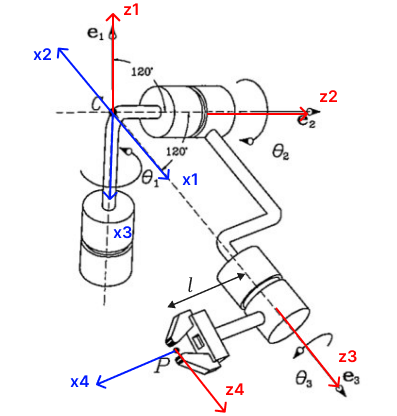
\includegraphics[width=0.4\textwidth]{figures/prob3.png}}
    \caption{Schematic view of the twist robot with its D-H vectors}
    \label{fig:prob3}
\end{figure}

\begin{table}[htbp]
    \caption{The D-H parameters of 3-DOF wrist robot}
    \def\arraystretch{1.25}
    \begin{center}
        \begin{tabular}{|Y|Y|Y|Y|Y|}
            \hline
            $i$ & $a_i$      & $b_i$ & $\alpha_i$ & $\theta_i$ \\
            \hline
            1   & 0          & 0     & $2\pi / 2$ & $\theta_1$ \\
            \hline
            2   & 0          & 0     & $2\pi / 3$ & $\theta_2$ \\
            \hline
            3   & \textit{l} & 0     & 0          & $\theta_3$ \\
            \hline
        \end{tabular}
    \end{center}
\end{table}

% \begin{small}
\begin{align*}
     & \left[Q_1\right] = \begin{bmatrix}
                              \cos \theta_1 & \frac{1}{2}\sin \theta_1   & \frac{\sqrt{3}}{2} \sin \theta_1   \\
                              \sin \theta_1 & -\frac{1}{2} \cos \theta_1 & - \frac{\sqrt{3}}{2} \cos \theta_1 \\
                              0             & \frac{\sqrt{3}}{2}         & -\frac{1}{2}
                          \end{bmatrix} \\
     & \left[Q_2\right] = \begin{bmatrix}
                              \cos \theta_2 & \frac{1}{2}\sin \theta_2   & \frac{\sqrt{3}}{2} \sin \theta_2   \\
                              \sin \theta_2 & -\frac{1}{2} \cos \theta_2 & - \frac{\sqrt{3}}{2} \cos \theta_2 \\
                              0             & \frac{\sqrt{3}}{2}         & -\frac{1}{2}
                          \end{bmatrix} \\
     & \left[Q_3\right] = \begin{bmatrix}
                              \cos \theta_3 & - \sin \theta_3 & 0 \\
                              \sin \theta_3 & \cos \theta_3   & 0 \\
                              0             & 0               & 1
                          \end{bmatrix}
\end{align*}
% \end{small}

So we can find $\vec{e}_i$ vectors and then, Jacobian matrix in the first joint frame, using equation \ref{eq:Jacobian}.
\begin{align*}
     & J_1 = [\mathbf{e_1}, \mathbf{e_2}, \mathbf{e_3}] \quad\quad & \text{where,} \quad\quad & [\mathbf{e}_1]_1 = [0, 0, 1]^T           \\
     & [\mathbf{e}_2]_1 = [Q_1][0, 0, 1]^T                         &                          & [\mathbf{e}_3]_1 = [Q_1][Q_2][0, 0, 1]^T
\end{align*}

\begin{align*}
     & \rightarrow J_1 =                                                                                                                                                                                                                                                                                                                                                                                                                                                                                                                                                                                                                                                                                                                                                                                                                                                                                     \\
     & \left(\begin{array}{ccc} 0 & \frac{\sqrt{3}\,\sin t_{1} }{2} & \frac{\sqrt{3}\,\cos t_{1} \,\sin t_{2} }{2}-\frac{\sqrt{3}\,\sin t_{1} }{4}-\frac{\sqrt{3}\,\cos t_{2} \,\sin t_{1} }{4}\\ 0 & -\frac{\sqrt{3}\,\cos t_{1} }{2} & \frac{\sqrt{3}\,\cos t_{1} }{4}+\frac{\sqrt{3}\,\cos t_{1} \,\cos t_{2} }{4}+\frac{\sqrt{3}\,\sin t_{1} \,\sin t_{2} }{2}\\ 1 & -\frac{1}{2} & \frac{1}{4}-\frac{3\,\cos t_{2} }{4} \end{array}\right)
\end{align*}


We can also write
\begin{align}
    [J]_1 = Q_1 [J]_2 \hspace{15px}\rightarrow\hspace{15px} [J]_2 = Q_1^T[J]_1
\end{align}

So, transferring our attained Jacobian to the second joint frame and substituting $\theta_1 \,\&\, \theta_2$ with $0 \,\&\, \pi/2$ gives \footnote{This result is achieved using MATLAB code. The code is also attached to this report file.}:

\begin{gather*}
    [J]_2 = \left(\begin{array}{ccc} 0 & 0 & \frac{\sqrt{3}}{2}\\ \frac{\sqrt{3}}{2} & 0 & 0\\ -\frac{1}{2} & 1 & -\frac{1}{2} \end{array}\right)
\end{gather*}

comparing it with the normalized version of given Jacobian matrix shows that they are totally similar. Then it's proved that the given Matrix is, indeed, the Jacobian of this robot.

\subsection{Calculating Force}
Using equation 5.50 0f the textbook \cite{b1}, we have:
\begin{gather}
    \mathbf{J}^T \mathbf{W} = \boldsymbol{\tau} \\
    \rightarrow \mathbf{W} = \mathbf{J}^{-T} \boldsymbol{\tau}
\end{gather}

where $\boldsymbol{\tau}$ is the 3-dimensional vector of joint forces and torques, whose \textit{i}-th component is $\tau_i$, whereas $\mathbf{W} = [\mathbf{n}^T , \mathbf{f}^T]$ denotes the wrench exerted by the environment on the EE, with \textbf{n} denoting the resultant moment and \textbf{f} the resultant force applied at point \textit{P} of the end-effector of the manipulator on Figure~\ref{fig:prob3}. So,

\begin{gather*}
    \begin{bmatrix}
        \mathbf{n} \\
        \mathbf{f}
    \end{bmatrix} = \left(\begin{array}{ccc} 0 & 0 & \frac{\sqrt{3}}{2}\\ \frac{\sqrt{3}}{2} & 0 & 0\\ -\frac{1}{2} & 1 & -\frac{1}{2} \end{array}\right)^{-T} \begin{bmatrix}
        20 \\
        20 \\
        -10
    \end{bmatrix} = \begin{bmatrix}
        0           \\
        20 \sqrt{3} \\
        20
    \end{bmatrix} \\
    \rightarrow \mathbf{n} = \begin{bmatrix}
        0      \\
        34.641 \\
        20
    \end{bmatrix}
\end{gather*}


\vspace{20px}
\section{Problem 4: Conceptual Analysis}
\subsection{Applications of Trajectory Planning}
\begin{enumerate}
    \item \textbf{Autonomous Vehicles (Self-Driving Cars)}: For autonomous vehicles to navigate safely and efficiently, trajectory planning is essential. It involves generating paths that avoid obstacles, follow traffic rules, and optimize fuel efficiency.
          \begin{itemize}
              \item \textit{Role and Purpose}: To ensure smooth and collision-free movement, allowing the vehicle to reach its destination while adhering to predefined constraints.
              \item \textit{Importance and Impact}: Proper trajectory planning avoids accidents, reduces travel time, improves passenger comfort, and enhances safety, especially in complex scenarios like lane changes, merging, and parking. Lack of planning means choosing simplest and fastest controlling routs which usually could lead to abrupt maneuvers, endangering passengers and other road users.
              \item \textit{Challenges}: Autonomous vehicles operate in dynamic environments with uncertainties (like sudden obstacles, road conditions, etc), requiring rapid trajectory adjustments. Real-time computation is challenging due to the need for quick decisions.
          \end{itemize}
    \item \textbf{Industrial Robots and Manufacturing}: In manufacturing environments, robots perform tasks like assembling, welding, painting, and material handling. Trajectory planning ensures smooth and accurate movements.
          \begin{itemize}
              \item \textit{Role and Purpose}: To ensure precise and efficient movements of industrial robots in manufacturing processes, avoiding collisions, optimizing cycle time, and maintaining product quality.
              \item \textit{Importance and Impact}: Optimized trajectories reduce production time, improve product quality, and minimize wear on robot components, while preventing collisions with workpieces, fixtures, or other robots. Without proper planning, robots may collide with objects, leading to damage and waste of energy.
              \item \textit{Challenges}: Industrial robots operate within confined spaces. Trajectory planning must consider workspace limitations. Avoiding collisions with static and moving obstacles (like other robots, conveyors, etc) is critical too. Robots can encounter singular configurations where certain joints lose motion capability. Handling these situations is challenging as well.
          \end{itemize}
    \item \textbf{Aerial Drones and Surveillance}: Drones rely on trajectory planning to navigate through airspace, capture images, and perform surveillance.
          \begin{itemize}
              \item \textit{Role and Purpose}: To avoid obstacles, maintain stable flight, and execute complex maneuvers (like search patterns, tracking moving targets, etc).
              \item \textit{Importance and Impact}: Precise trajectories enhance image quality during surveillance missions. Quadcopters are also sometimes used for irrigation, manuring, or spraying pesticides; to cover the entire agricultural land, a thorough trajectory must be designed to minimize the costs and energy.
              \item \textit{Challenges}: Balancing trajectory efficiency with battery life is challenging. Detecting and avoiding dynamic obstacles (like birds, other drones, etc) and adapting to the ever-changing climate and wind requires robust algorithms.
          \end{itemize}
\end{enumerate}

% \vspace{20px}
\subsection{Trajectory Planning Methods}
\begin{itemize}
    \item \textbf{Autonomous Vehicles (Self-Driving Cars)}
          \begin{enumerate}
              \item \textit{Polynomial Trajectory Planning}: To follow a smooth path while driving a car, this method can be used, enhancing the passenger comfort and avoiding sudden accelerations.
              \item \textit{Point-to-Point Trajectory Planning}: To reach from a starting point to the destination point on the road, the fastest way, this method might be used. Since it causes sudden steering and rapid speed changes, it's not appropriate for on-road travels. It might be of use in special cases like race cars or military vehicles.
          \end{enumerate}
    \item \textbf{Industrial Robots and Manufacturing}
          \begin{enumerate}
              \item \textit{Minimum Jerk Trajectory}: This method must be used for applications where not only must no force be applied at the beginning or ending of a robot's motion, but also there must be no jerk at these moments.
              \item \textit{Cycloidal Motion}: This method is quite much same as \textit{Polynomial Interpolation} methods; meaning it has zero velocity and acceleration (and thus, force) at the start and end of the motion. But it applies high jerks at the start and stop moments. So it is a simple and practical method for applications with less sensitivity and affectivity.
          \end{enumerate}
    \item \textbf{Aerial Drones and Surveillance}
          \begin{enumerate}
              \item \textit{Trapezoidal Velocity Profile}: This method creates a simple velocity profile which starts at zero, reaches a respectively long constant maximum and ends at zero. This creates a respectively smooth motion, although not as much as what 3-4-5 or 4-7 polynomials do.
              \item \textit{Rectangular Velocity Profile}: The simplest way to plan a motion is to hold the required speed from beginning to the end, with no alternation. This is a not practical motion for most of the applications, since they need a smooth and jerk-less motion to avoid harming the objects or the robot itself. However, in military applications like armed drones, this method might be of use, since it's able to perform the fastest motions and satisfy the rapid maneuvers expected from a military vehicle. Since these drones are equipped with highly durable materials and devices, this method can cause no harm to their actuators and systems \cite{b7}.
          \end{enumerate}
\end{itemize}

\subsection{Optimization and Metrics}
\subsubsection*{I) Trajectory Optimization Methods}
\begin{enumerate}
    \item \textbf{Model Predictive Path Integral (MPPI)}:
          \begin{itemize}
              \item \textbf{Overview}: MPPI combines path integral control with model predictive control (MPC).
              \item \textbf{Working Principle}: MPPI leverages path integral control theory to compute solutions for stochastic optimal control. It optimizes a finite-horizon trajectory at each time step, sampling trajectories and evaluating them using a cost function. MPPI adapts to changing environments and disturbances, providing real-time solutions.
              \item \textbf{Impacts}:
                    \begin{itemize}
                        \item \textbf{Smooth Trajectories}: MPPI minimizes jerk (rate of acceleration change), resulting in smoother motion profiles.
                        \item \textbf{Adaptability}: It handles dynamic environments effectively.
                        \item \textbf{Real-Time Performance}: MPPI provides timely trajectory adjustments \cite{b3}.
                    \end{itemize}
          \end{itemize}

    \item \textbf{Optimal Trajectory Generation with Jerk Minimization}:
          \begin{itemize}
              \item \textbf{Objective}: Minimize jerk along the trajectory.
              \item \textbf{How It Works}:
                    \begin{itemize}
                        \item \textbf{Cost Function}: Formulate a cost function that penalizes jerk.
                        \item \textbf{Optimization}: Solve an optimization problem to find a trajectory with minimized jerk.
                        \item \textbf{Constraints}: Consider collision avoidance, velocity limits, and dynamic feasibility.
                    \end{itemize}
              \item \textbf{Impacts}:
                    \begin{itemize}
                        \item \textbf{Smooth Motion}: Reduced jerk leads to smoother profiles.
                        \item \textbf{Energy Efficiency}: Lower jerk reduces energy consumption.
                        \item \textbf{Comfort}: Enhances passenger comfort.
                        \item \textbf{Safety}: Avoids sudden acceleration changes \cite{b4}.
                    \end{itemize}
          \end{itemize}
\end{enumerate}

\subsubsection*{II) Metrics for Evaluating Trajectory Performance}
\begin{itemize}
    \item \textbf{Smoothness}:
          \begin{itemize}
              \item \textbf{Jerk}: Evaluate acceleration change rate. Smoother trajectories have lower jerk.
              \item \textbf{Curvature}: Assess directional changes. Smaller curvature indicates smoother paths.
          \end{itemize}

    \item \textbf{Efficiency}:
          \begin{itemize}
              \item \textbf{Energy Consumption}: Measure energy required to follow the trajectory.
              \item \textbf{Time}: Consider execution time; faster trajectories are more efficient \cite{b6}.
          \end{itemize}

    \item \textbf{Safety}:
          \begin{itemize}
              \item \textbf{Collision Avoidance}: Ensure trajectory avoids obstacles.
              \item \textbf{Dynamic Feasibility}: Adherence to system dynamics and constraints.
          \end{itemize}

    \item \textbf{Accuracy}:
          \begin{itemize}
              \item \textbf{Goal Achievement}: Evaluate how well the trajectory reaches desired goals.
              \item \textbf{Tracking Error}: Measure deviation from the desired path.
          \end{itemize}

    \item \textbf{Robustness}:
          \begin{itemize}
              \item \textbf{Sensitivity Analysis}: Assess sensitivity to disturbances or uncertainties.
              \item \textbf{Adaptability}: Evaluate handling of unexpected changes.
          \end{itemize}
\end{itemize}

\section{Problem 5: Trajectory Generation}
\begin{figure}[H]
    \centerline{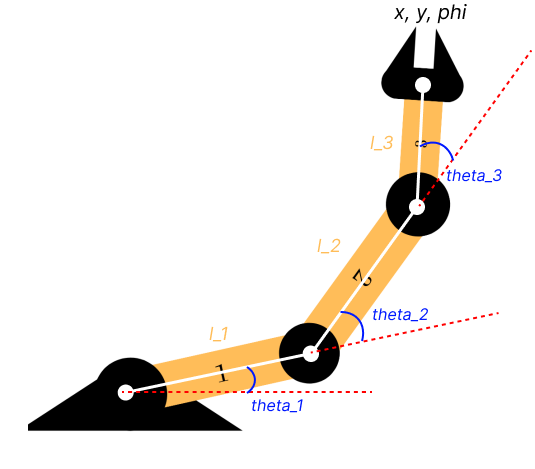
\includegraphics[width=0.4\textwidth]{figures/prob5.png}}
    \caption{Planar 3-DOF robot with its angles marked up}
    \label{fig:prob5}
\end{figure}

\subsection{Forward and inverse kinematics}
FKP Equations: Having $\theta_1$, $\theta_2$ and $\theta_3$, we want to find $x, y$ and $\phi$ of end-effector.
\begin{align}
     & x     = l_1 \cos \theta_1 + l_2 \cos (\theta_1 + \theta_2) + l_3 \cos (\theta_1 + \theta_2 + \theta_3) \\
     & y    = l_1 \sin \theta_1 + l_2 \sin (\theta_1 + \theta_2) + l_3 \sin (\theta_1 + \theta_2 + \theta_3)  \\
     & \phi  = \theta_1 + \theta_2 + \theta_3
\end{align}

IKP Equations: Having $x, y$ and $\phi$ of end-effector, we want to find $\theta_1$, $\theta_2$ and $\theta_3$.
\begin{align*}
     & x            = l_1 \cos \theta_1 + l_2 \cos (\theta_1 + \theta_2) + l_3 \cos \phi                         \\
     & y            = l_1 \sin \theta_1 + l_2 \sin (\theta_1 + \theta_2) + l_3 \sin \phi                         \\
     & \rightarrow (x - l_1 \cos \theta_1 - l_3 \cos \phi)^2 + (y - l_1 \sin \theta_1 - l_3 \sin \phi)^2 = l_2^2
\end{align*}

\begin{gather}
    A \cos \theta_1 + B \sin \theta_1 = C \label{eq:IKP} \\
    A = 2 l_1 (x - l_3 \cos \phi)         \\
    B = 2 l_1 (y - l_3 \sin \phi)         \\
    C = x^2 + y^2 + l_1^2 - l_2^2 + l_3^2 - 2 l_3 (x \cos \phi + y \sin \phi)
\end{gather}

\begin{large}
    \begin{align*}
         & Answers \longrightarrow
        \begin{cases}
            \theta_1 ^+ \longrightarrow\theta_2 ^+ \longrightarrow \theta_3 ^+ \\[30pt]
            \theta_1 ^- \longrightarrow\theta_2 ^- \longrightarrow \theta_3 ^-
        \end{cases}
    \end{align*}
\end{large}

\subsection{Angular pose, velocity and acceleration equations}
General form of equations for angle, angular velocity, acceleration and jerk comes from:
\begin{align}
    \vec{\theta}(t)         & = \vec{\theta}_i + \left(\vec{\theta}_f - \vec{\theta}_i\right) s(\tau) \label{eq:angle} \\
    \dot{\vec{\theta}}(t)   & = \frac{1}{T} \left(\vec{\theta}_f - \vec{\theta}_i\right) s'(\tau)                      \\
    \ddot{\vec{\theta}}(t)  & = \frac{1}{T^2} \left(\vec{\theta}_f - \vec{\theta}_i\right) s''(\tau)                   \\
    \dddot{\vec{\theta}}(t) & = \frac{1}{T^3} \left(\vec{\theta}_f - \vec{\theta}_i\right) s'''(\tau)
\end{align}
where, for each of the trajectory planning methods, the linear slope function $s(\tau)$ is derived according to the course pamphlet as below.
\vspace{3px}

\subsubsection{\textbf{Trapezoidal Polynomial}}
\begin{itemize}
    \item conditions: \begin{footnotesize}
              \(s(0) = s'(0) = 0; s(1) = 1, s'(1) = 0\)
          \end{footnotesize}
    \item maximum order of linear polynomial: 3
    \item achieved polynomial: \(\underline{\mathbf{s(\tau) = - 2\tau^3 + 3\tau^2}}\)
\end{itemize}

\vspace{11px}

\subsubsection{\textbf{3-4-5 Interpolating Polynomial}}
\begin{itemize}
    \item conditions: \begin{footnotesize}\(s(0) = s'(0) = s''(0) = 0; s(1) = 1, s'(1) = s''(1) = 0\) \end{footnotesize}
    \item maximum order of linear polynomial: 5
    \item achieved polynomial: \(\underline{\mathbf{s(\tau) = 6\tau^5 - 15\tau^4 + 10\tau^3}}\)
\end{itemize}

\vspace{11px}

\subsubsection{\textbf{4-5-6-7 Interpolating Polynomial}}
\begin{itemize} % \renewcommand{\labelitemi}{} % -> Remove the bullet
    \item conditions: \begin{footnotesize}\(s(0) = s'(0) = s''(0) = s'''(0) = 0; s(1) = 1, s'(1) = s''(1) = s'''(0) = 0\) \end{footnotesize}
    \item maximum order of linear polynomial: 7
    \item achieved polynomial: \\
          \(\underline{\mathbf{s(\tau) = -20\tau^7 + 70\tau^6 - 84\tau^5 + 35\tau^4}}\)
\end{itemize}

\vspace{11px}

\subsubsection{\textbf{Polynomial-Based 3-point Trajectory}}
Assuming the robot is to meet the intermediate point \textit{B} at instant: \\
\(t=1(s) \rightarrow \tau = 1/2\)

\begin{itemize}
    \item  conditions: \begin{footnotesize}
              \(s(0) = s'(0) = s''(0) = 0; s(0.5) = S; s(1) = 1, s'(1) = s''(1) = 0\)
          \end{footnotesize}
          \textit{where we can find \textbf{S} from:} \(\theta(0.5) = \theta^I + \left(\theta^F - \theta^I\right) S \)
    \item maximum order of linear polynomial: 6
    \item achieved polynomial: \\
          \(\underline{\mathbf{s(\tau) = 27.13\tau^6 - 75.40\tau^5 + 66.40\tau^4 - 17.13\tau^3}}\)
\end{itemize}

% \begin{enumerate}
%     \item \textbf{Trapezoidal Method}: conditions: \(s(0) = s'(0) = 0; s(1) = 1, s'(1) = 0\) \\
%           maximum order of linear Polynomial: 3 \\
%           achieved Polynomial: \(s(\tau) = - 2\tau^3 + 3\tau^2\)
%     \item \textbf{3-4-5 Interpolating Polynomial}: conditions: \(s(0) = s'(0) = s''(0) = 0; s(1) = 1, s'(1) = s''(1) = 0\) \\
%           maximum order of linear Polynomial: 5 \\
%           achieved Polynomial: \(s(\tau) = 6\tau^5 - 15\tau^4 + 10\tau^3\)
%     \item \textbf{4-5-6-7 Interpolating Polynomial}: conditions: \(s(0) = s'(0) = s''(0) = s'''(0) = 0; s(1) = 1, s'(1) = s''(1) = s'''(0) = 0\) \\
%           maximum order of linear Polynomial: 7 \\
%           achieved Polynomial: \(s(\tau) = -20\tau^7 + 70\tau^6 - 84\tau^5 + 35\tau^4\)
%     \item \textbf{Polynomial-based 3-point trajectory}: assuming the robot is to meet the intermediate point \textit{B} at instant \(t=1s \rightarrow \) conditions: \(s(0) = s'(0) = s''(0) = 0; s(0.5) = z; s(1) = 1, s'(1) = s''(1) = 0\) \\
%           where we can find value \textit{z} from: \(\vec{\theta}(t=0.5) = \vec{\theta}_i + \left(\vec{\theta}_f - \vec{\theta}_i\right) s(\tau)\)
%           maximum order of linear Polynomial: 7 \\
%           achieved Polynomial: \(s(\tau) = -20\tau^7 + 70\tau^6 - 84\tau^5 + 35\tau^4\)
% \end{enumerate}

Note that for the last method, to meet all of the three required points, we need a somehow different prospect. The polynomial trajectories discussed for the first three methods do not allow the specification of intermediate Cartesian poses of the EE. All they guarantee is that the Cartesian trajectories prescribed at the initial and final instants are met \cite{b1}. One way of verifying the feasibility of the Cartesian trajectories is with what are called \textbf{via poses}, i.e., poses of the EE in the Cartesian space that lie between the initial and the final poses, and are determined so as to avoid collisions \cite{b8}.
Using \textit{via pose}, requires finding the joint space of the robot to access the intermediate point (B in this case), via IKP. The following shows how this is done, using equation \ref{eq:IKP} and its relative sub-equations.
\begin{align*}
    \text{pt.} B:\quad & x_{EE} = 1.0774L,\quad y_{EE} = 0.4673L,\quad \phi_{EE} = 30^\circ         \\
    l_1 = \,           & l_2 = \frac{3}{2}l_3 = L \rightarrow                                       \\
    A = \,             & 2L(1.0774L - \frac{2}{3}L \times \frac{\sqrt{3}}{2}) = L^2                 \\
    B = \,             & 2L(0.4673L - \frac{2}{3}L \times \frac{1}{2}) = 0.2679L^2                  \\
    C = \,             & (1.0774L)^2 + (0.4673L)^2 + (\frac{2}{3}L)^2 - 2\cdot\frac{2}{3}L \, \cdot \\
                       & (1.0774L \frac{\sqrt{3}}{2} + 0.4673L \frac{1}{2}) = 0.2679L^2
\end{align*}
\begin{large}
    \setlength{\abovedisplayshortskip}{-4pt}
    \setlength{\belowdisplayshortskip}{-4pt}
    \[
        \rightarrow \, \cos (\theta_1) + 0.2679 \, \sin (\theta_1) = 0.2679
    \]
\end{large}
\begin{align*}
     & \rightarrow \, \theta_1^+ = 1.5708 rad = 90^\circ \quad\quad & \theta_1^- = -1.0473 rad = -60^\circ \\
     & \rightarrow \, \theta_2^+ = -2.6179 rad = -150^\circ         & \theta_2^- = 2.6179 rad = 150^\circ  \\
     & \rightarrow \, \theta_3^+ = 1.5707 rad = 90^\circ            & \theta_3^- = -1.0471 rad = -60^\circ \\
\end{align*}
\hrule
\begin{align*}
    \text{pt.} & A:\quad x_{EE} = 1.3660L,\quad y_{EE} = 2.0327L,\quad \phi_{EE} = 90^\circ \\
               & A = 1.3987 L^2 \quad B = 2.7321 L^2 \quad C = 3.7320 L^2                   \\
               & \rightarrow \,1.3987 \cos (\theta_1) + 2.7321 \, \sin (\theta_1) =  3.7320
\end{align*}
\begin{align*}
     & \rightarrow \, \theta_1^+ = 83.14^\circ  & \theta_1^- = -8.96^\circ \\
     & \rightarrow \, \theta_2^+ = -66.47^\circ & \theta_2^- = 85.0^\circ  \\
     & \rightarrow \, \theta_3^+ = 73.33^\circ  & \theta_3^- = 13.96^\circ \\
\end{align*}
\hrule
\begin{align*}
    \text{pt.} & C:\quad  x_{EE} = -0.6994L,\quad y_{EE} = 1.9434L,\quad \phi_{EE} = 120^\circ \\
               & A = -0.3988 L^2 \quad B = 2.1547 L^2 \quad C = 0.6449 L^2                     \\
               & \rightarrow \, -0.3988 \cos (\theta_1) + 2.1547 \, \sin (\theta_1) =  0.6449
\end{align*}
\begin{align*}
     & \rightarrow \, \theta_1^+ = 173.37^\circ  & \theta_1^- = 27.60^\circ  \\
     & \rightarrow \, \theta_2^+ = -110.00^\circ & \theta_2^- = 116.61^\circ \\
     & \rightarrow \, \theta_3^+ = 56.64^\circ   & \theta_3^- = -24.21^\circ \\
\end{align*}


According to the source book \cite{b1}, \textit{Chapter 6.5, p267-269}, for one intermediate point, \textit{B}, we must consider one joint, for example first joint ($\theta_1$), and use its value, (\textit{attained from IKP}), in a scalar version of equation \ref{eq:angle}. So,
\begin{gather*}
    @ t = 1(s) \rightarrow \tau = 1/2 \rightarrow s(1/2) = S\\
    \theta(1/2) = \theta^I + \left(\theta^F - \theta^I\right) S \\
    \theta(1/2) = \theta_1^B \quad\quad \theta^I = \theta_1^A \quad\quad \theta^F = \theta_1^C \rightarrow \\
    90 = 83.14 + (173.37 - 83.14) s(\tau = 1/2)
\end{gather*}

\vspace{15px}
This adds a new constraint to the $s(\tau)$ which is: \(s(\tau=0.5) = S\). We already had 6 other conditions as we had in \textit{3-4-5 Polynomial} method, which were:
\(s(0) = s'(0) = s''(0) = 0; s(1) = 1, s'(1) = s''(1) = 0\).
Overall, there are 7 conditions our Interpolating Polynomial must satisfy, so it can be a linear polynomial of maximum order of 6. So,
\[s(\tau) = a\tau^6 + b\tau^5 + c\tau^4 + d\tau^3 + e\tau^2 + f\tau + g\]
Applying these conditions gives:
\begin{align*}
     & g = f = e = 0 ; \quad\quad\quad\quad\quad\, a + b + c + d = 1 ;                         \\
     & 6a + 5b + 4c + 3d = 0 ; \quad\quad 30a + 20b + 12c + 6d = 0 ;                           \\
     & a(\frac{1}{2})^6 + b(\frac{1}{2})^5 + c(\frac{1}{2})^4 + d(\frac{1}{2})^3 = 0.0760279 ;
\end{align*}

Solving this system of linear equations gives:
\begin{gather*}
    a = 27.13 \quad b = -75.40 \quad c =  66.40 \quad d = -17.13 \\
    \underline{\mathbf{s(\tau) = 27.13\, \tau^6 - 75.40\, \tau^5 + 66.40\, \tau^4 - 17.13\, \tau^3}}
\end{gather*}


\subsection{Plotting the velocity profiles}
In this section, MATLAB is used to plot multiple diagrams. First, \(s(\tau)\) and its derivatives are plotted for each of the 4 methods discussed. The first derivative indicates the \emph{velocity} profile, the second derivative indicates the \emph{acceleration} profile and the third one, corresponds to \emph{jerk} parameter. Note that the first method, \textit{Trapezoidal} profile, has two figures: first one models a trapezoid with a Polynomial of third degree, while the second one creates a precise sharp trapezoid, using \textit{heaviside} function.\footnote{Assuming the trajectory is divided to three equal sections: accelerating to maximum speed of \(S = 1 rad/s\), keeping the constant speed and decelerating to stop at the end point of the path.}

The \textbf{Heaviside step function}, denoted as \(H(x)\), is a mathematical function. It behaves like a switch, returning different values based on its input:
\begin{itemize}
    \item For \(x < 0\), \(H(x)\) is 0.
    \item For \(x = 0\), \(H(x)\) is \(\frac{1}{2}\).
    \item For \(x > 0\), \(H(x)\) is 1.
\end{itemize}

Using heaviside function, we can create a trapezoidal shape for \underline{velocity} relation like: \textit{($S =$ maximum speed)}
\begin{align*}
     & s'(\tau) = \begin{cases}
                      S \cdot \tau  & \quad\quad 0 < \tau < \frac{1}{3}           \\[15pt]
                      S             & \quad\quad \frac{1}{3} < \tau < \frac{2}{3} \\[15pt]
                      -S \cdot \tau & \quad\quad \frac{1}{3} < \tau < 1
                  \end{cases}
\end{align*}

The results are exactly as expected, satisfying the velocity, acceleration and jerk values at the beginning and ending of each trajectory. After that, the joint space information is thoroughly plotted using $\theta_i$s and their derivatives for each method. Again the Trapezoidal Method is divided to \textit{sharp} and \textit{soft} methods. The results are represented in Figures~\ref{fig:res1} to \ref{fig:res6} in the Appendix.

\subsection{Comparison of velocity profiles}
\begin{enumerate}
    \item 3-4-5 Polynomial: \begin{itemize}
              \item This trajectory method uses a polynomial curve with coefficients corresponding to the degrees 3, 4, and 5.
              \item The velocity profile exhibits smooth transitions, but it may not handle high speeds well.
              \item The maximum velocity during the rise period is moderate1.
          \end{itemize}
    \item 4-5-6-7 Polynomial: \begin{itemize}
              \item This method extends the polynomial curve to include coefficients for degrees 4, 5, 6, and 7.
              \item It achieves zero jerk (rate of change of acceleration) and finite fourth-order characteristics.
              \item However, note that the maximum velocity and acceleration within the rise period have increased compared to the 3-4-5 polynomial12.
          \end{itemize}
    \item Trapezoidal Method: \begin{itemize}
              \item The trapezoidal method combines constant acceleration and deceleration.
              \item It ensures zero velocity at both ends of the rise period.
              \item The resulting motion curve consists of two parabolas, providing smoother transitions.
              \item However, the maximum acceleration remains discontinuous at the start and end of the rise portion1.
          \end{itemize}
    \item Via Pose Method: \begin{itemize}
              \item The via pose method involves specifying intermediate poses (waypoints) for the robot.
              \item It constructs a trajectory that passes through these waypoints.
              \item While it allows flexibility in defining desired poses, the velocity profile depends on the specific waypoints chosen13.\cite{b9}
          \end{itemize}
\end{enumerate}

\subsection{Practicality of last method}
As discussed in the classroom, the way we handled the last method in order to cross a mid-point in the trajectory is straight-forward, but very limited. In fact, this method uses system of \underline{linear} equations that might seem easy for few mid-points on the trajectory, but as this number increases, the complexity and volume of computations get exponentially huge and huger. So no driver or PLC would be able to handle it for real-world multi-point applications. That's why so many have been introducing via-pose methods to ease this process. These methods are beyond the syllabus of this course and this homework report.



\section{Problem 6: MATLAB Coding}
In this problem, pre-written MATLAB commands are used to generate different trajectories for passing through provided path points. To use these functions, some additional libraries must have been installed on MATLAB like \textit{Robotics System Toolbox}. \cite{b10}

For installing the mentioned toolbox, the following procedure has been followed.
\subsection{Installation from shared MATLAB Drive}
This will work for MATLAB Online or MATLAB Desktop provided you have MATLAB drive setup.

\begin{itemize}
    \item Click on the appropriate link below and an invitation to share will be emailed to the address associated with your MATLAB account:\begin{itemize}
              \item RVC 2nd edition RTB10+MVTB4 (2017)
              \item RVC 1st edition: RTB9+MVTB3 (2011)
          \end{itemize}
    \item Accept the invitation.
    \item A folder named RVC1 or RVC2 will appear in your MATLAB drive folder.
    \item Use the MATLAB file browser and navigate to the folder RVCx/rvctools and double-click the script named startup\_rvc.m
    \item Note that this is a combo-installation that includes the Machine Vision Toolbox (MVTB) as well.
    \item Type \texttt{rtbdemo} in command prompt to see if the library has been successfully installed and is running well. \cite{b11}
\end{itemize}

\vspace{10px}
\subsection{Implementation of programs}
Two series of codes are provided for this problem. First one is a thorough unit code named prob6.m which includes the whole program. The other is a combination of \textit{Matlab Live Script} files\footnote{suffixed as .mlx file} which provide the implementation of each of the required methods, separately and in a different way, requiring correct installation of mentioned toolboxes which might not be accessible in some devices. Both series are appended along this report. The results can be found in Figures~\ref{fig:res7} to \ref{fig:res10} in the Appendix.

\vspace{10px}
\subsection{Discussion on peak velocities and accelerations}
Peak velocity and acceleration are key parameters in trajectory planning methods, influencing the efficiency, stability, and safety of motion profiles. In the Multi-Point Trapezoidal method, peak velocity represents the maximum speed attained between waypoints, occurring at the midpoint of each segment, while peak acceleration denotes the highest rate of change of velocity, typically at the segment boundaries. These parameters help ensure smooth transitions and adherence to system constraints. In Multi-Point Cubic Polynomials, peak velocity and acceleration similarly characterize maximum speed and rate of change of velocity, but with smoother trajectories due to cubic polynomial interpolation. Quintic polynomials further refine trajectory smoothness, potentially lowering peak velocity and acceleration while maintaining precision. Understanding and optimizing peak velocity and acceleration enable engineers to design motion profiles that meet performance requirements, minimize stress on mechanical components, and ensure stable, efficient motion.

\vspace{10px}
\subsection{Discussion on trajectory planning methods}

The first three methods of trajectory planning —\textit{Multi-Point Trapezoidal}, \textit{Multi-Point Cubic Polynomials}, and \textit{Multi-Point Quintic Polynomials}— differ primarily in their mathematical representation of the trajectory and the resulting characteristics of the generated paths. Let's discuss each method's key features:

\begin{enumerate}
    \item \textbf{Multi-Point Trapezoidal:}
          \begin{itemize}
              \item \textbf{Description:} This method divides the trajectory into segments with trapezoidal velocity profiles. Each segment consists of a ramp-up, constant velocity, and ramp-down phase, resembling the shape of a trapezoid.
              \item \textbf{Mathematical Representation:} The trajectory is represented by a series of straight-line segments with constant acceleration and deceleration.
              \item \textbf{Characteristics:}
                    \begin{itemize}
                        \item Simple to implement and computationally efficient.
                        \item Generates trajectories with constant acceleration and deceleration, resulting in smooth transitions between waypoints.
                        \item Suitable for applications where simplicity and predictable motion are preferred over higher-order path planning.
                    \end{itemize}
          \end{itemize}

    \item \textbf{Multi-Point Cubic Polynomials:}
          \begin{itemize}
              \item \textbf{Description:} This method generates trajectories using cubic polynomial functions. These functions smoothly interpolate between waypoints by fitting a cubic polynomial to each segment of the trajectory.
              \item \textbf{Mathematical Representation:} The trajectory is represented by a set of cubic polynomial functions, where each function defines a segment between consecutive waypoints.
              \item \textbf{Characteristics:}
                    \begin{itemize}
                        \item Provides more flexibility in shaping the trajectory compared to trapezoidal profiles.
                        \item Produces trajectories with continuous velocity and acceleration profiles, resulting in smoother motion.
                        \item Requires solving systems of linear equations to compute polynomial coefficients, which may introduce computational overhead compared to trapezoidal profiles.
                    \end{itemize}
          \end{itemize}

    \item \textbf{Multi-Point Quintic Polynomials:}
          \begin{itemize}
              \item \textbf{Description:} This method extends the cubic polynomial approach by using quintic (degree-five) polynomial functions to generate trajectories. Quintic polynomials offer additional degrees of freedom, allowing for even smoother path transitions and better handling of constraints.
              \item \textbf{Mathematical Representation:} The trajectory is represented by a set of quintic polynomial functions, providing higher-order continuity between waypoints.
              \item \textbf{Characteristics:}
                    \begin{itemize}
                        \item Offers superior smoothness and continuity compared to cubic polynomials, particularly in terms of higher-order derivatives such as jerk.
                        \item Enables more precise control over trajectory shaping and adherence to constraints such as velocity and acceleration limits.
                        \item Requires solving more complex systems of equations compared to cubic polynomials, potentially leading to increased computational complexity.
                    \end{itemize}
          \end{itemize}
\end{enumerate}

\subsection{Discussion on differences of methods}
The primary distinction between the B-spline method and the other three methods (Multi-Point Trapezoidal, Multi-Point Cubic Polynomials, and Multi-Point Quintic Polynomials) lies in their trajectory representation. While the former employs piecewise polynomial curves of higher degrees for interpolation, the latter methods use simpler functions like straight lines or lower-degree polynomials. This difference impacts robot performance by offering B-splines smoother paths and better adaptability to complex constraints and environments. However, B-splines entail higher computational complexity, potentially affecting real-time performance in dynamic settings. Therefore, the choice depends on balancing the need for trajectory flexibility and smoothness with computational resources and real-time constraints in robot applications.

\subsection{Discussion on use cases of methods}
Multi-Point Trapezoidal trajectories are ideal for operations needing efficient and predictable motion, like manufacturing assembly lines, due to their simplicity and computational efficiency, ensuring rapid execution while maintaining stability. Conversely, B-spline trajectories suit tasks requiring precise and smooth motion, such as robotic surgeries or autonomous vehicle navigation, offering superior flexibility and adaptability to complex environments, enhancing performance and safety in challenging scenarios.

\subsection{Overall conclusion of trajectory planning}
Trajectory generation in robotics is a crucial aspect influencing performance and efficiency. Different methods, such as Multi-Point Trapezoidal and B-splines, offer unique advantages based on task complexity and computational resources. While simpler methods suffice for straightforward operations, complex techniques like B-splines are preferred for precise motion in intricate environments. Understanding these methods' strengths and limitations is key to designing effective robotic systems tailored to specific applications.

\vspace{50px}
\section{Conclusion}
\textbf{
    In conclusion, this report delves into the significance of Jacobians in robotics and control theory. These mathematical tools elucidate the relationship between joint velocities and end-effector velocities. Additionally, our analysis encompasses trajectory planning, a crucial aspect of determining feasible paths for robots. MATLAB plays a pivotal role in implementing these concepts, allowing us to create smooth trajectories, explore polynomial paths, and optimize motion profiles. We will indeed keep exploring these fascinating areas to enhance robotic control and automation!
}
\vspace{20px}

\begin{thebibliography}{00}
    \bibitem{b1} J. Angeles, ``Fundamentals of Robotic Mechanical Systems'', Theory, Methods, and Algorithms, 4th edition, Springer.

    \bibitem{b2} J. J. Craig, ``Introduction to Robotics'', 3d edition, Pearson Education, Inc.

    \bibitem{b3} M. Kazim, J. Hong, M. Kim, K. K. Kim, (2023). ``Recent advances in path integral control for trajectory optimization: An overview in theoretical and algorithmic perspectives''. Annual Reviews in Control, 57, 100931. [Online]. Available: \url{https://doi.org/10.1016/j.arcontrol.2023.100931}

    \bibitem{b4} B. Nadir, O. Mohammed, N. Minh-Tuan, et al. ``Optimal trajectory generation method to find a smooth robot joint trajectory based on multiquadric radial basis functions''. Int J Adv Manuf Technol 120, 297-312 (2022). [Online]. Available: \url{https://doi.org/10.1007/s00170-022-08696-1}

    \bibitem{b5} M. Ceccarelli, M. Russo, (2020). ``Parallel Architectures for Humanoid Robots''. Robotics, 9(4). [Online]. Available: \url{https://doi.org/10.3390/robotics9040075}

    \bibitem{b6} T. Stouraitis, L. Yan, J. Moura, M. Gienger and S. Vijayakumar, ``Multi-mode Trajectory Optimization for Impact-aware Manipulation,'' 2020 IEEE/RSJ International Conference on Intelligent Robots and Systems (IROS), Las Vegas, NV, USA, 2020, pp. 9425-9432, doi: 10.1109/IROS45743.2020.9341246.

    \bibitem{b7} R. Liebhart, ``Navigating the World of Robotics: Rectangular vs. Trapezoidal Motion Profiles'', MAB Robotics. [Online]. Available: \url{http://bit.ly/3U8IkDu}

    \bibitem{b8} Gosselin, C.M., and Hadj-Messaoud, A., 1993, “Automatic planning of smooth trajectories for
    pick-and-place operations”, ASME Journal of Mechanical Design, Vol. 115, no. 3, pp. 450-456.

    \bibitem{b9} T. Kirana, S. K. Srivastavab, ``Analysis and Simulation of Cam Follower Mechanism Using Polynomial Cam Profile'', International Journal of Multidisciplinary and Current Research. [Online]. Available: \url{http://ijmcr.com/wp-content/uploads/2013/11/Paper15211-2151.pdf}

    \bibitem{b10} MATLAB documentation, ``Trajectory Generation'', MathWorks.com, \url{https://www.mathworks.com/help/robotics/trajectory-generation.html}

    \bibitem{b11} P. Corke, ``robotics-toolbox-matlab'', Github, \url{https://github.com/petercorke/robotics-toolbox-matlab?tab=readme-ov-file#install-from-shared-matlab-drive-folder}
\end{thebibliography}

% -------------------------------------------------------------
\vspace{30px}
\section{Appendix}
\subsection{Resulted Plots of Problem 5: six figures}
\begin{figure}[htbp]
    \centering
    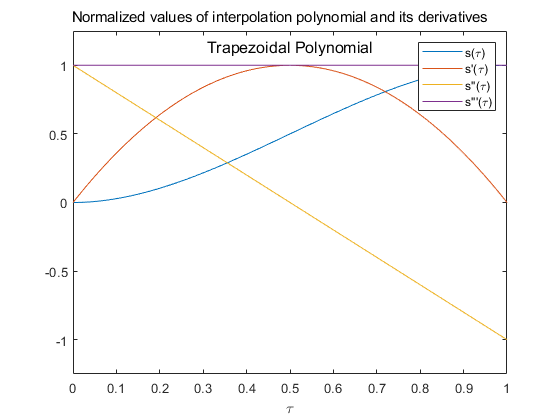
\includegraphics[width=0.35\textwidth]{figures/prob5/s(tau)/1.png}
    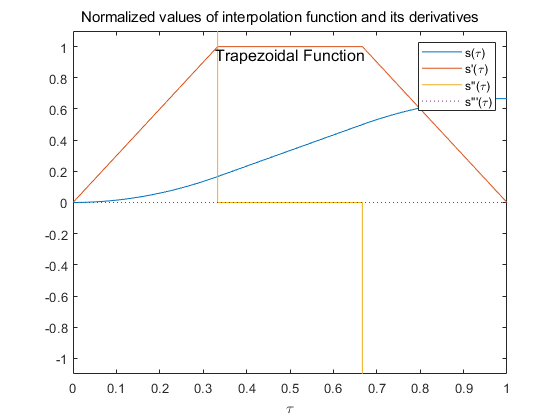
\includegraphics[width=0.35\textwidth]{figures/prob5/s(tau)/2.png}
    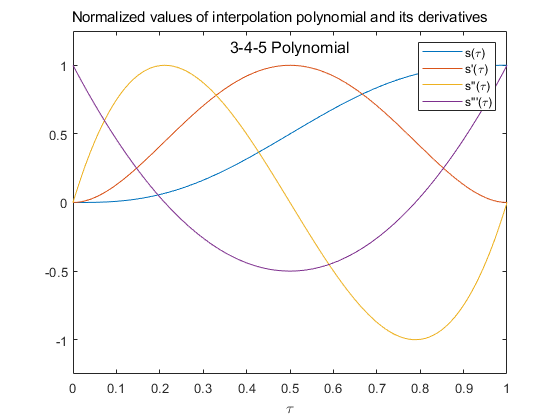
\includegraphics[width=0.35\textwidth]{figures/prob5/s(tau)/3.png}
    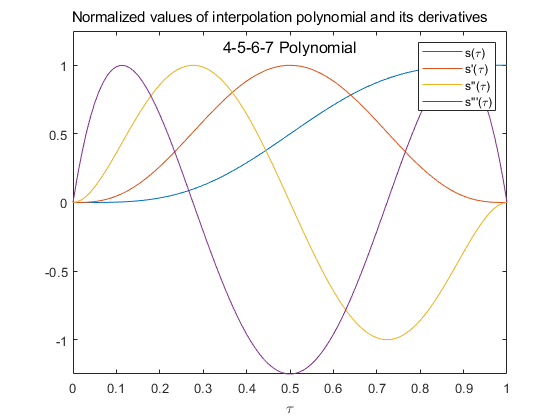
\includegraphics[width=0.35\textwidth]{figures/prob5/s(tau)/4.png}
    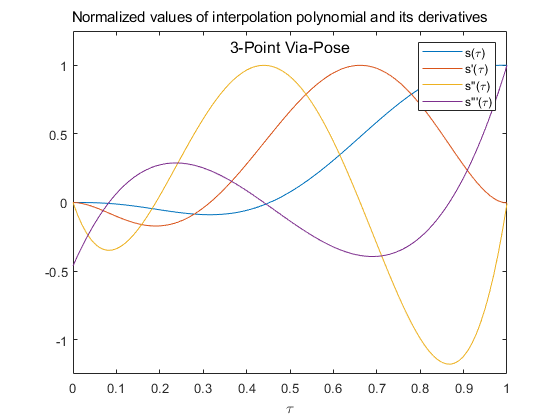
\includegraphics[width=0.35\textwidth]{figures/prob5/s(tau)/5.png}
    \caption{Interpolating functions ($s(\tau)$) and their derivatives based on operation time for 5 pre-described methods}
    \label{fig:res1}
\end{figure}

\begin{figure}[htbp]
    \centering
    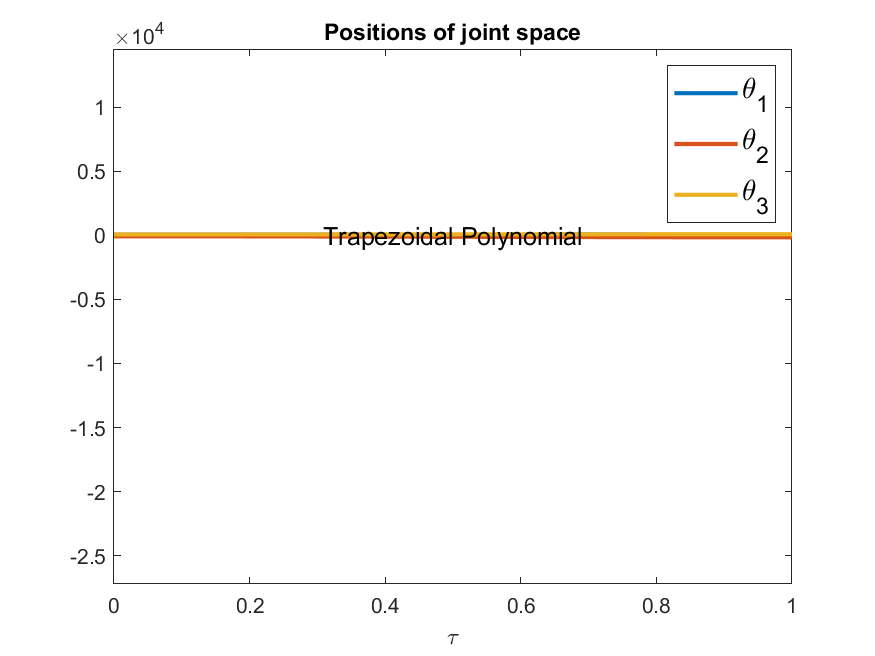
\includegraphics[width=0.4\textwidth]{figures/prob5/theta_i/position_Trapezoidal Polynomial.png}
    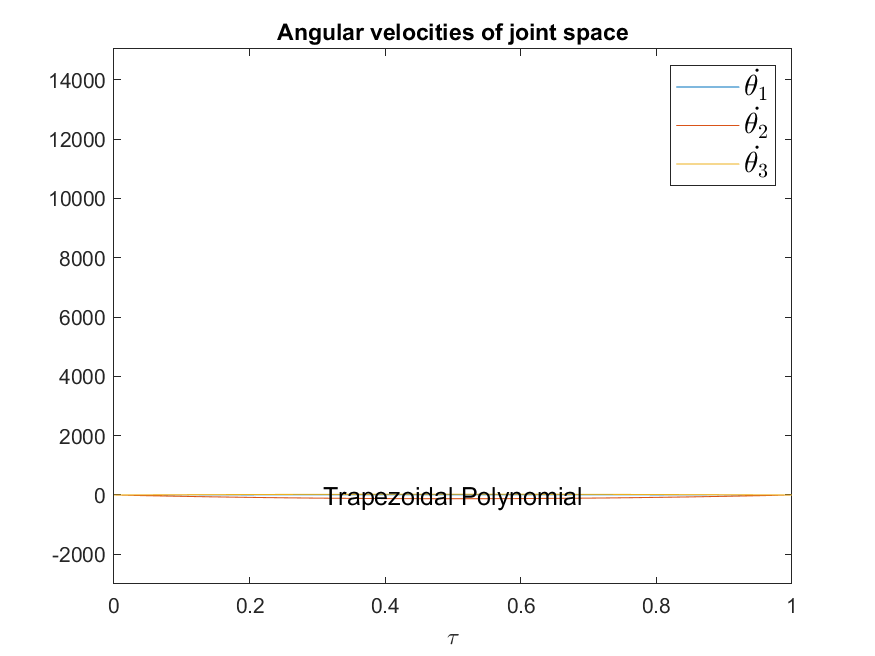
\includegraphics[width=0.4\textwidth]{figures/prob5/theta_i/velocity_Trapezoidal Polynomial.png}
    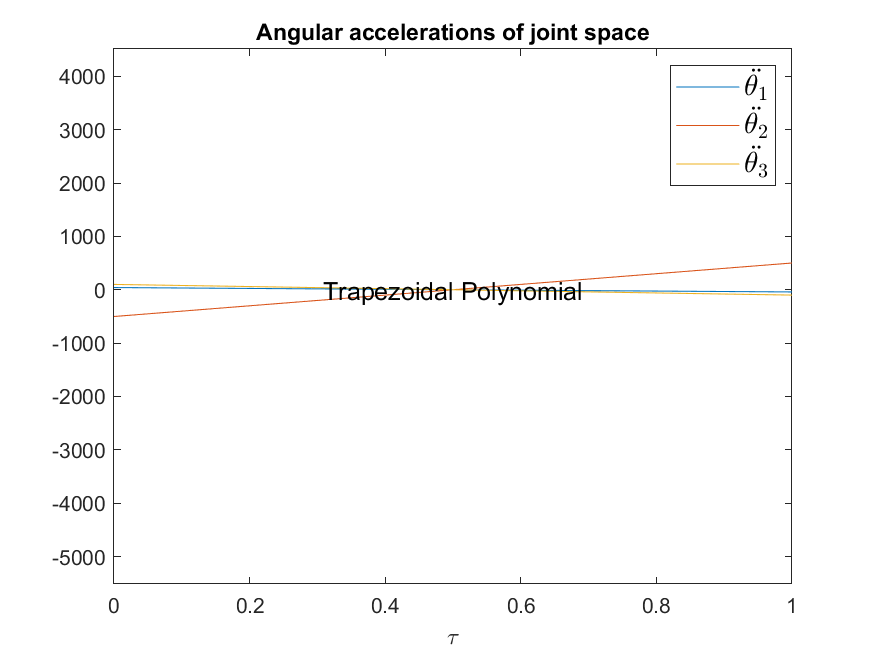
\includegraphics[width=0.4\textwidth]{figures/prob5/theta_i/acceleration_Trapezoidal Polynomial.png}
    \caption{Angular position, velocity and acceleration for Semi-Trapezoidal trajectory based on operation time}
    \label{fig:res2}
\end{figure}

\begin{figure}[htbp]
    \centering
    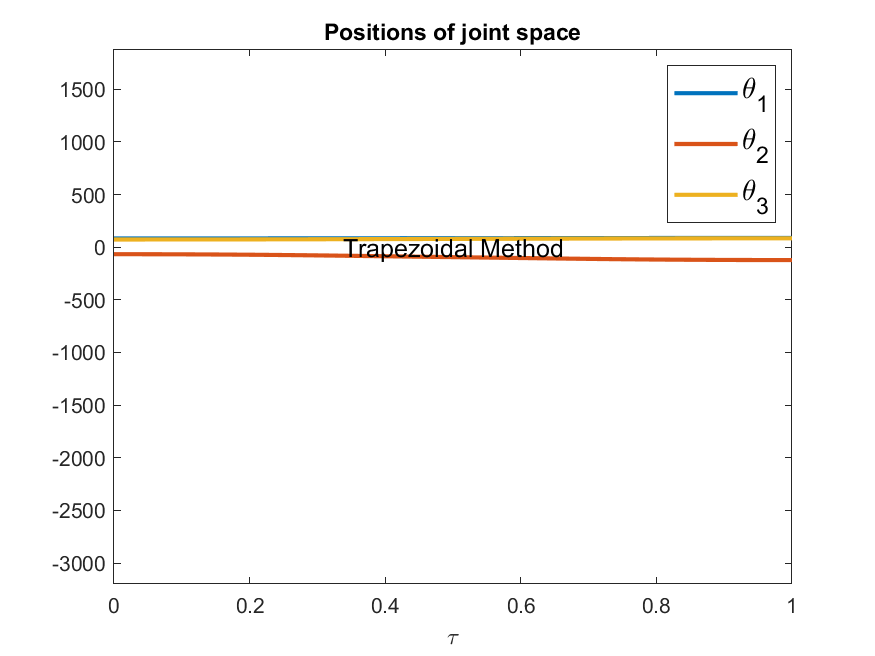
\includegraphics[width=0.4\textwidth]{figures/prob5/theta_i/position_Trapezoidal Method.png}
    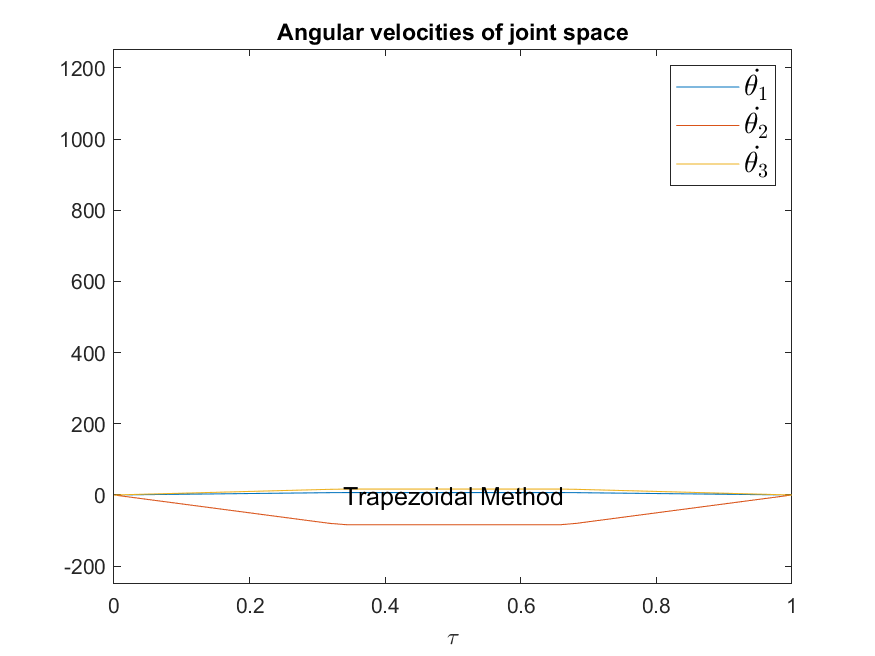
\includegraphics[width=0.4\textwidth]{figures/prob5/theta_i/velocity_Trapezoidal Method.png}
    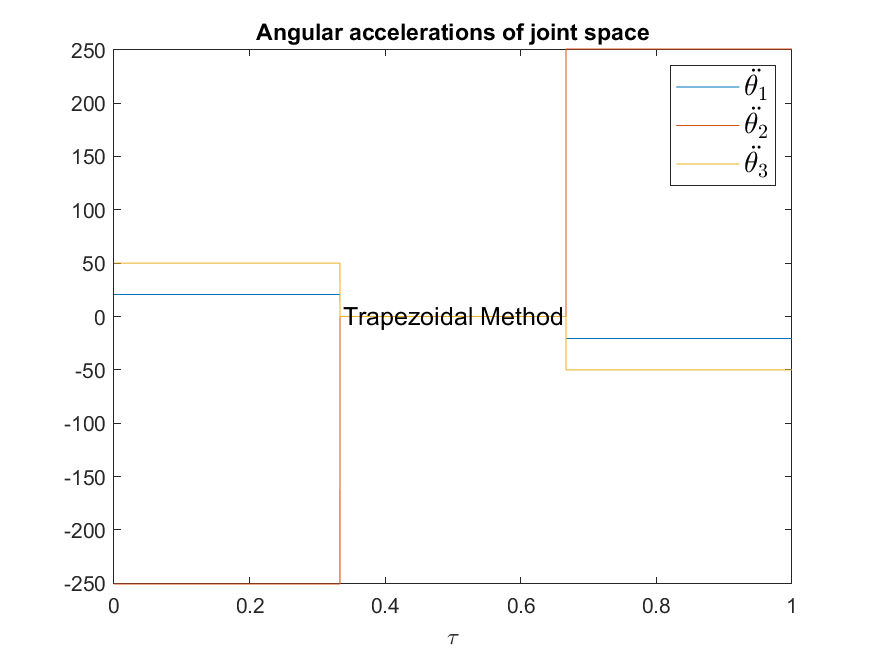
\includegraphics[width=0.4\textwidth]{figures/prob5/theta_i/acceleration_Trapezoidal Method.png}
    \caption{Angular position, velocity and acceleration for Sharp Trapezoidal trajectory based on operation time}
    \label{fig:res3}
\end{figure}

\begin{figure}[htbp]
    \centering
    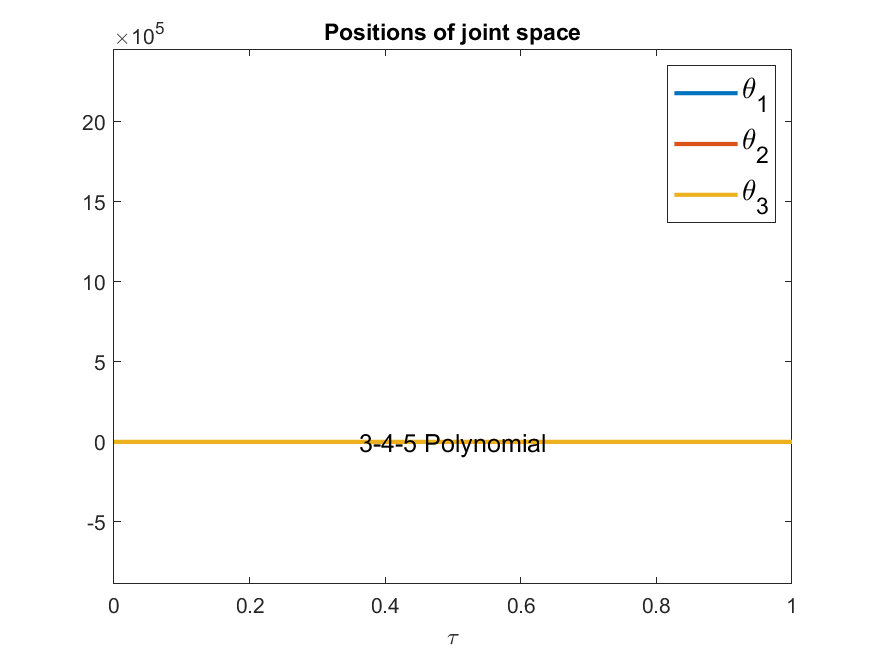
\includegraphics[width=0.4\textwidth]{figures/prob5/theta_i/position_3-4-5 Polynomial.png}
    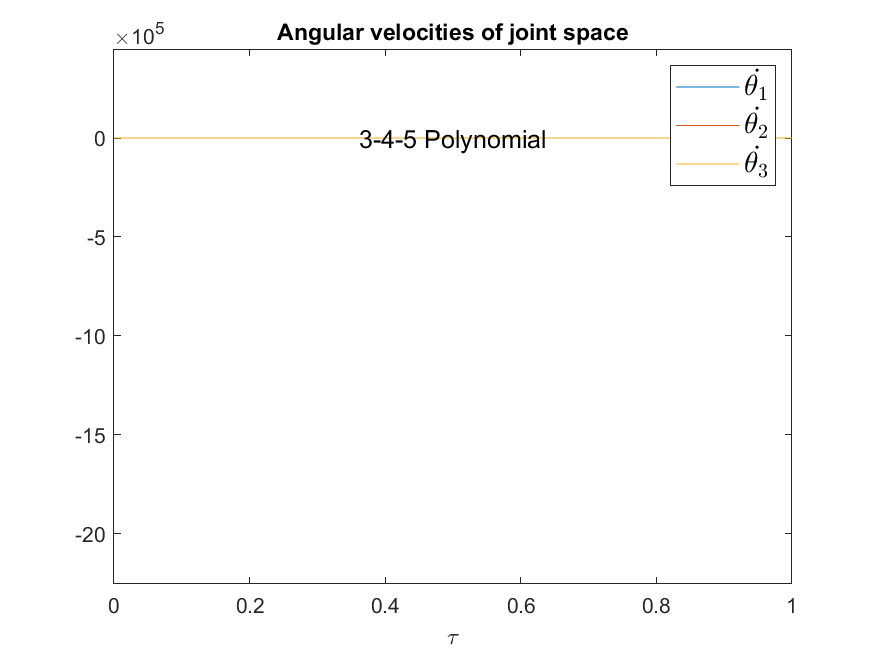
\includegraphics[width=0.4\textwidth]{figures/prob5/theta_i/velocity_3-4-5 Polynomial.png}
    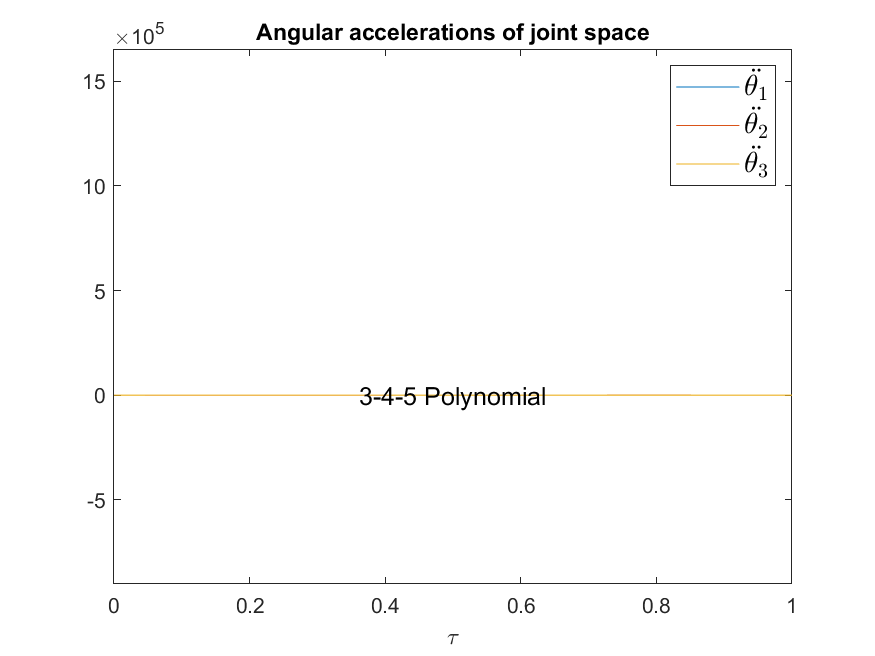
\includegraphics[width=0.4\textwidth]{figures/prob5/theta_i/acceleration_3-4-5 Polynomial.png}
    \caption{Angular position, velocity and acceleration for 3-4-5 trajectory based on operation time}
    \label{fig:res4}
\end{figure}

\begin{figure}[htbp]
    \centering
    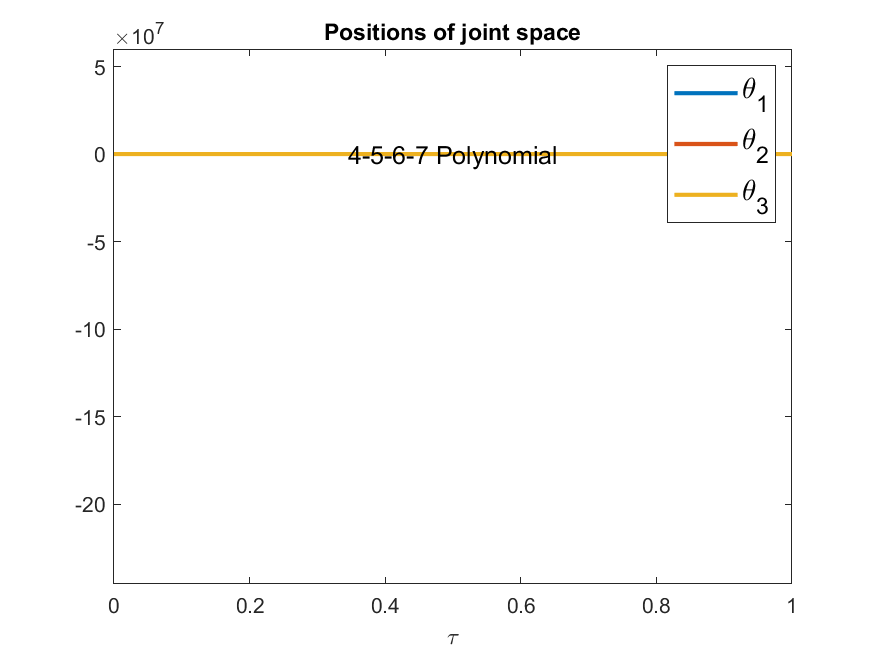
\includegraphics[width=0.4\textwidth]{figures/prob5/theta_i/position_4-5-6-7 Polynomial.png}
    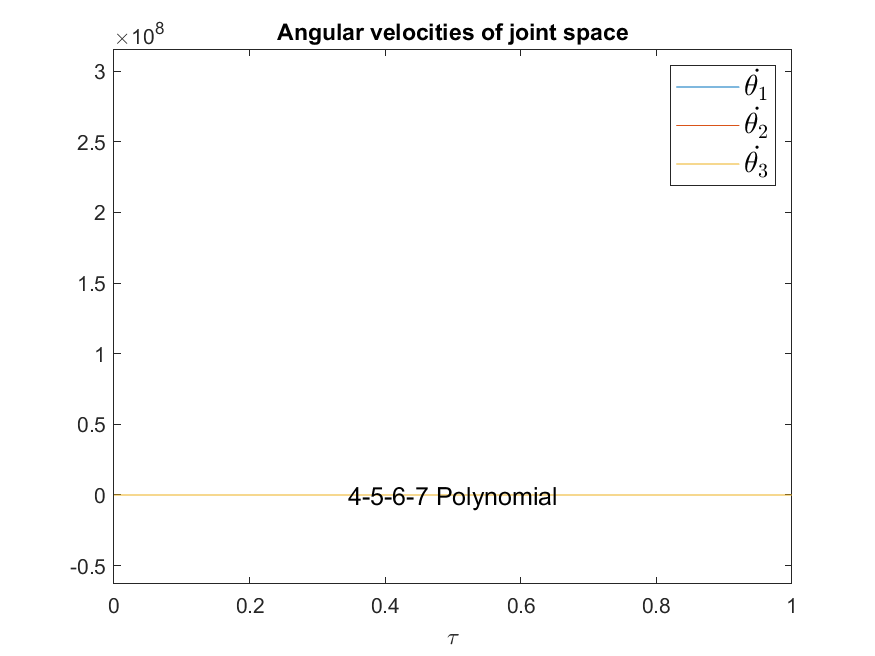
\includegraphics[width=0.4\textwidth]{figures/prob5/theta_i/velocity_4-5-6-7 Polynomial.png}
    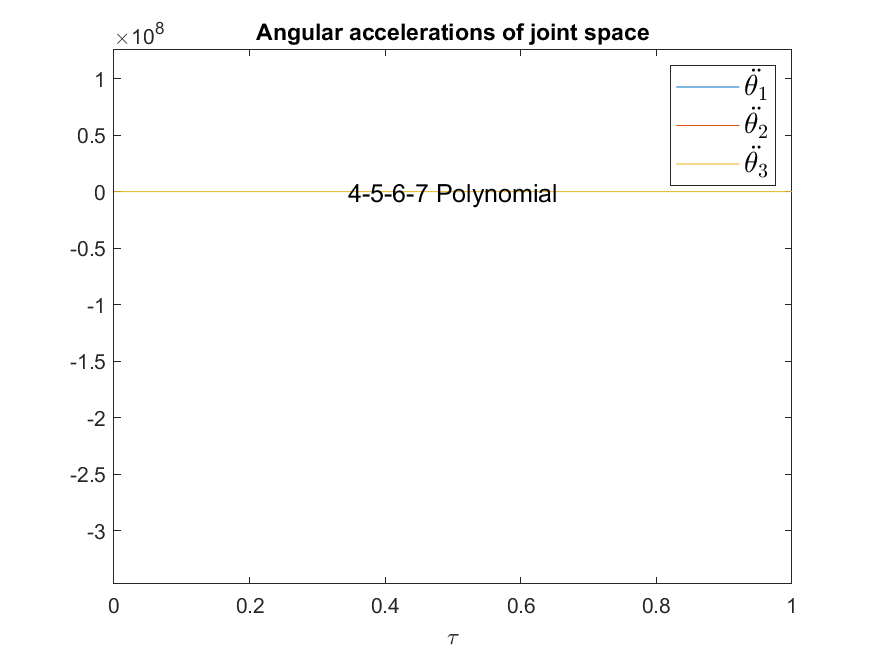
\includegraphics[width=0.4\textwidth]{figures/prob5/theta_i/acceleration_4-5-6-7 Polynomial.png}
    \caption{Angular position, velocity and acceleration for 4-5-6-7 trajectory based on operation time}
    \label{fig:res5}
\end{figure}

\begin{figure}[htbp]
    \centering
    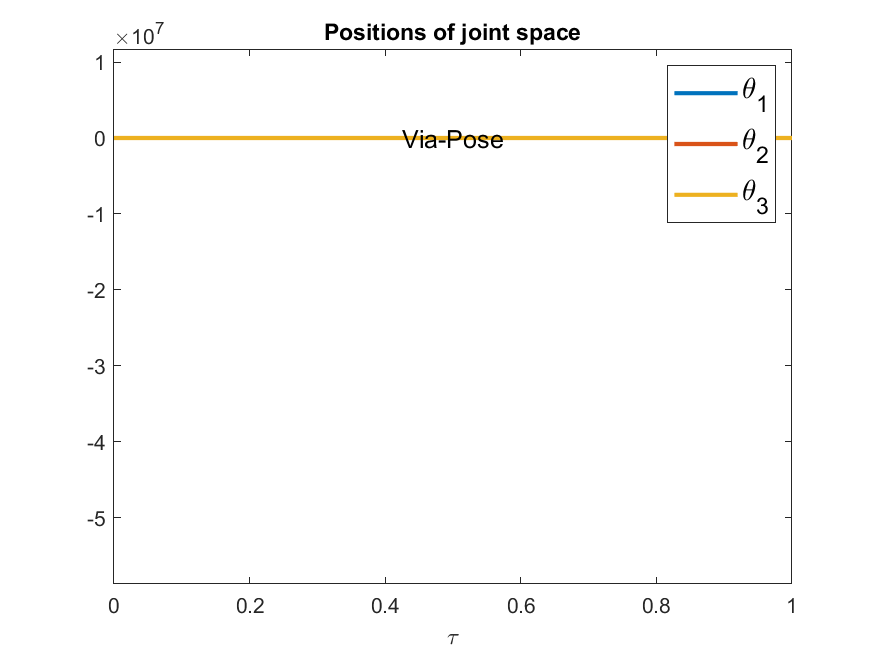
\includegraphics[width=0.4\textwidth]{figures/prob5/theta_i/position_Via-Pose.png}
    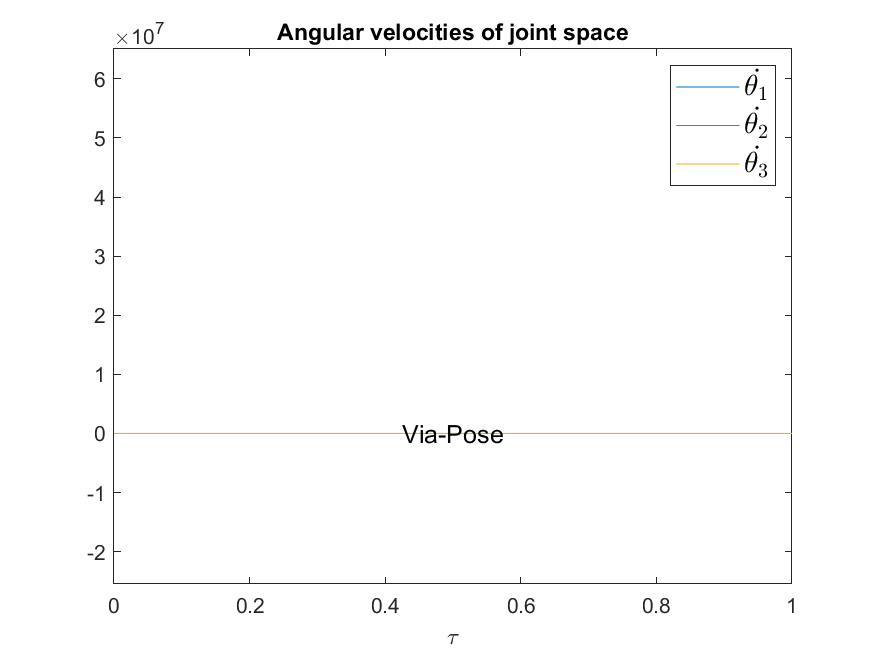
\includegraphics[width=0.4\textwidth]{figures/prob5/theta_i/velocity_Via-Pose.png}
    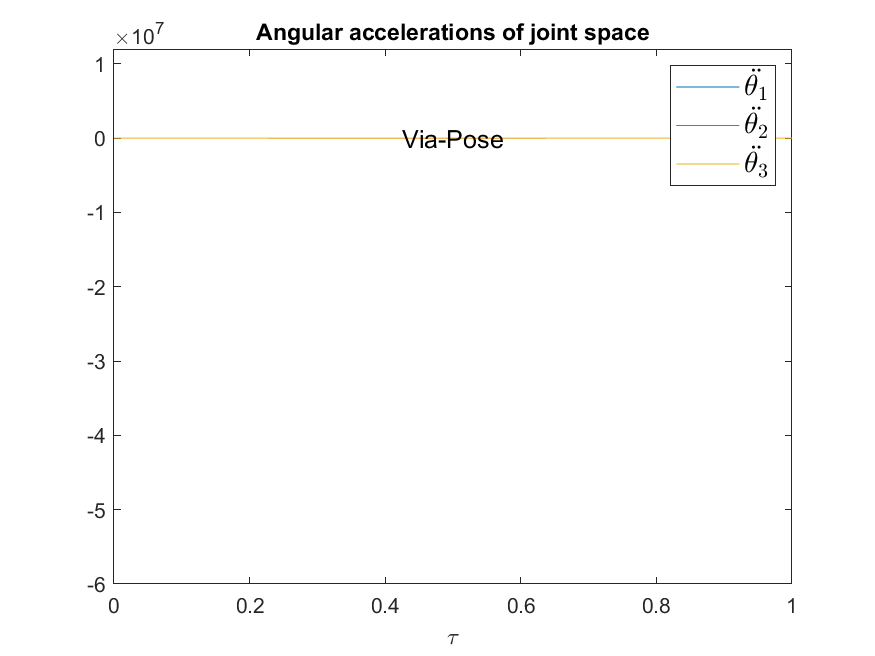
\includegraphics[width=0.4\textwidth]{figures/prob5/theta_i/acceleration_Via-Pose.png}
    \caption{Angular position, velocity and acceleration for 3-point via-pose trajectory based on operation time}
    \label{fig:res6}
\end{figure}

\subsection{Resulted Plots of Problem 6: four figures}
\begin{figure}[htbp]
    \centering
    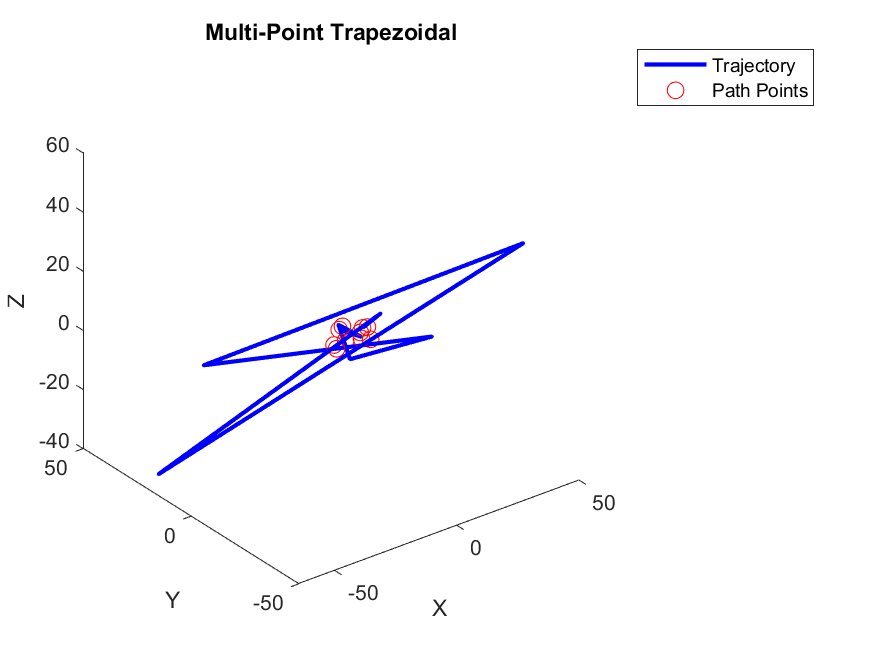
\includegraphics[width=0.4\textwidth]{figures/prob6/fig_1.png}
    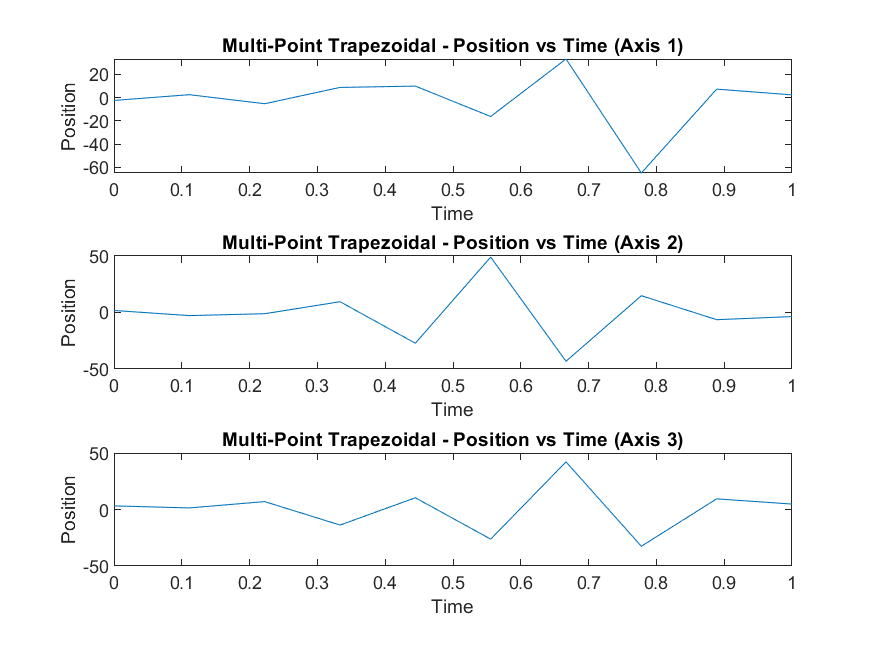
\includegraphics[width=0.4\textwidth]{figures/prob6/fig_2.png}
    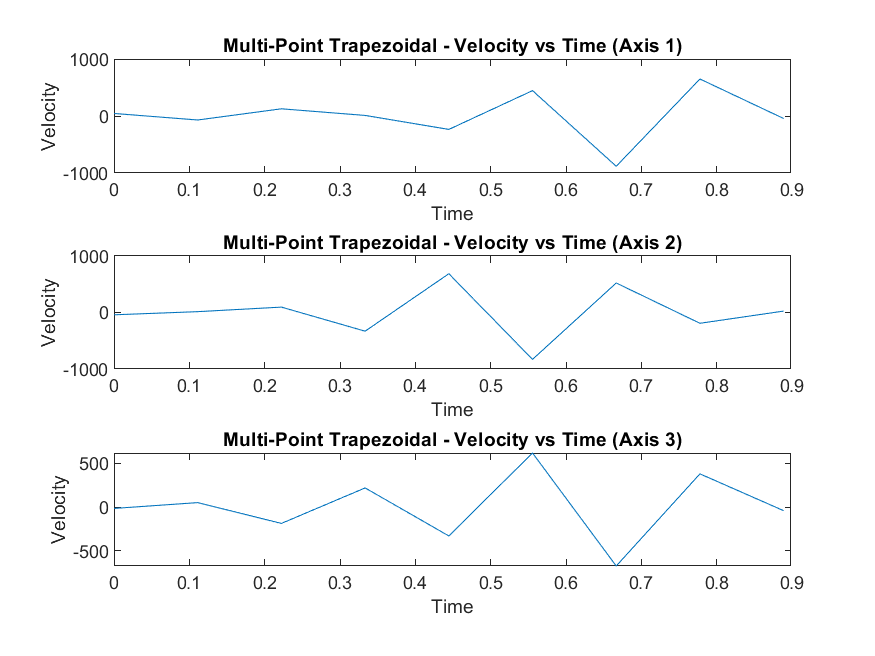
\includegraphics[width=0.4\textwidth]{figures/prob6/fig_3.png}
    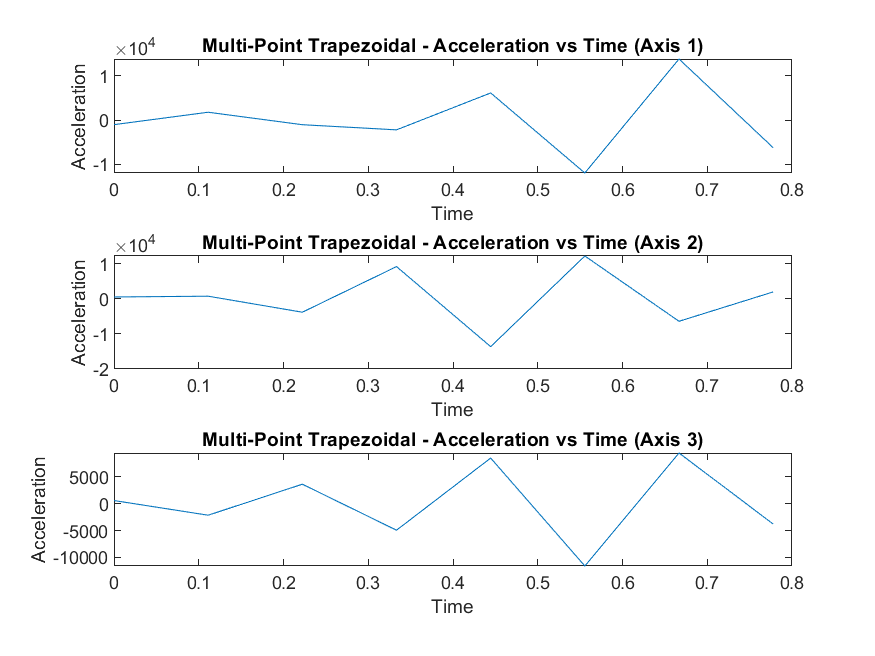
\includegraphics[width=0.4\textwidth]{figures/prob6/fig_4.png}
    \caption{First four results for problem 6}
    \label{fig:res7}
\end{figure}

\begin{figure}[htbp]
    \centering
    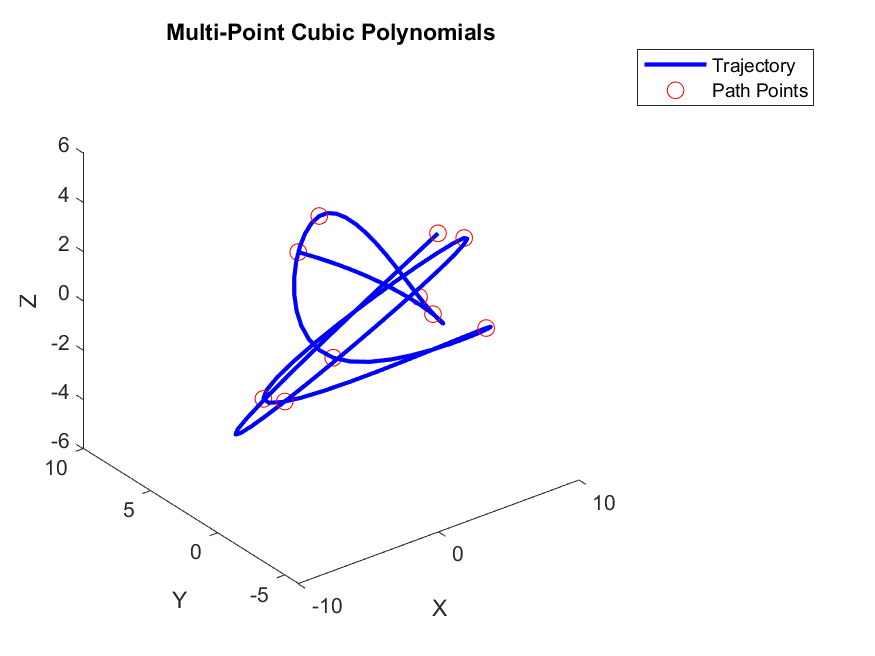
\includegraphics[width=0.4\textwidth]{figures/prob6/fig_5.png}
    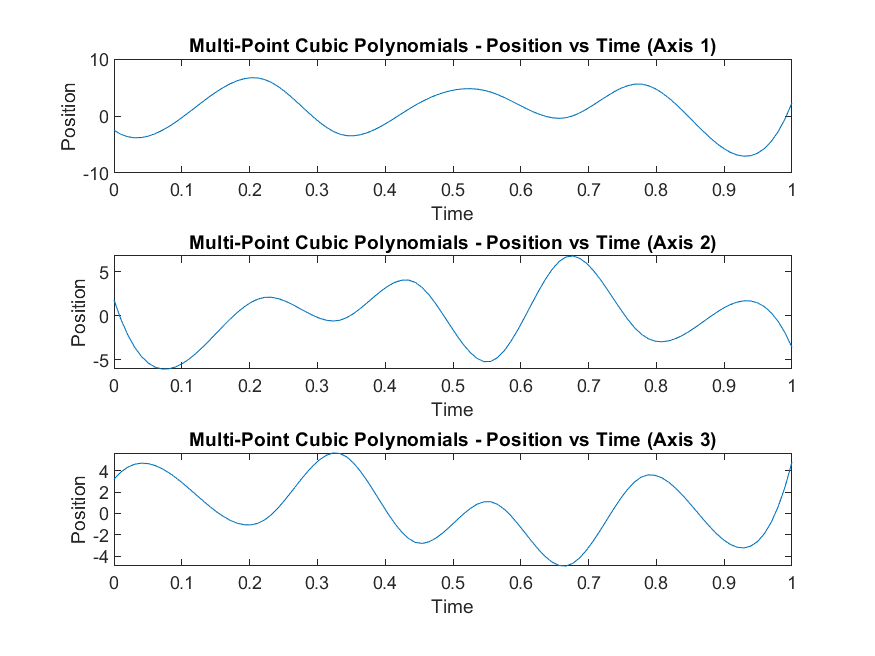
\includegraphics[width=0.4\textwidth]{figures/prob6/fig_6.png}
    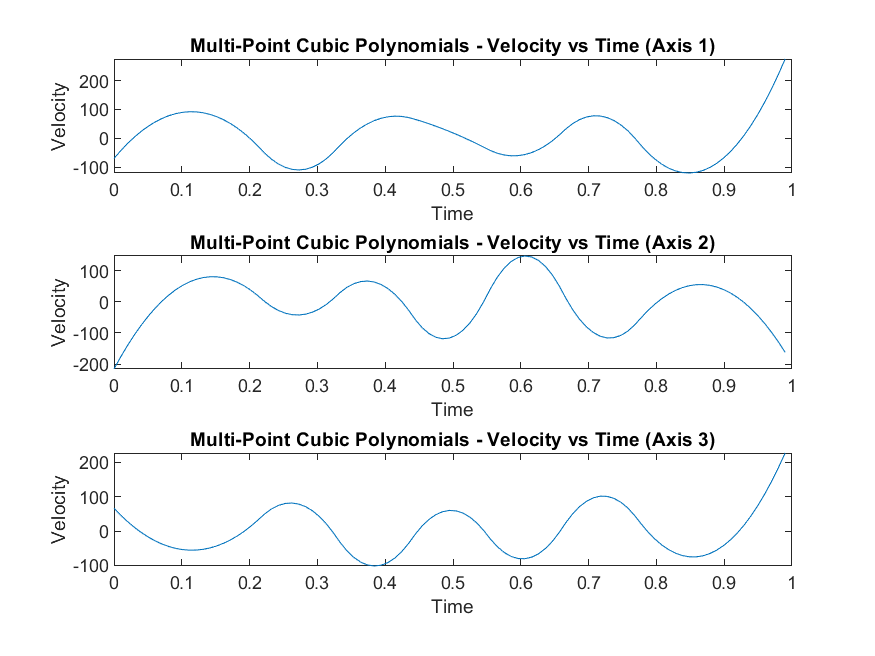
\includegraphics[width=0.4\textwidth]{figures/prob6/fig_7.png}
    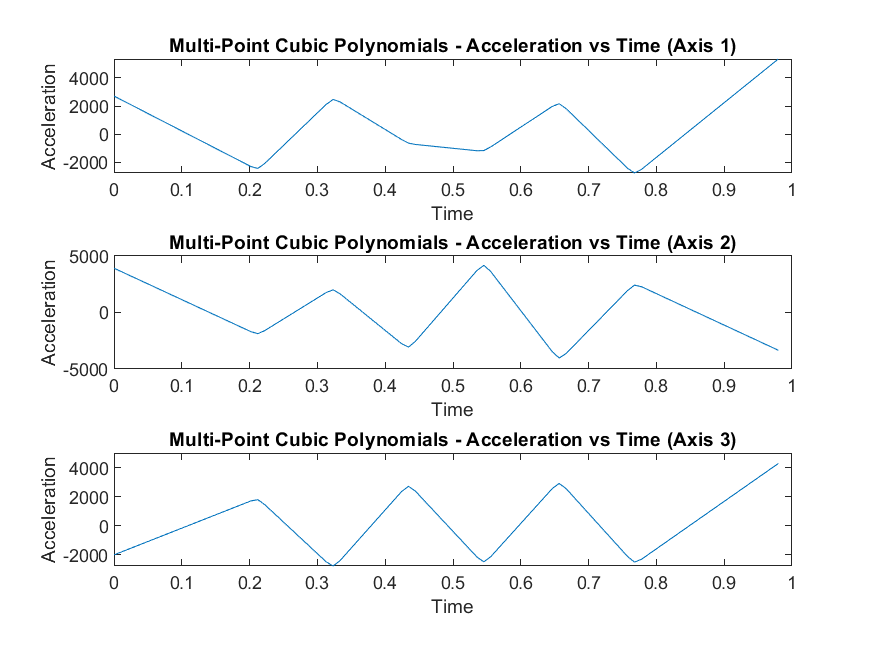
\includegraphics[width=0.4\textwidth]{figures/prob6/fig_8.png}
    \caption{Second four results for problem 6}
    \label{fig:res8}
\end{figure}

\begin{figure}[htbp]
    \centering
    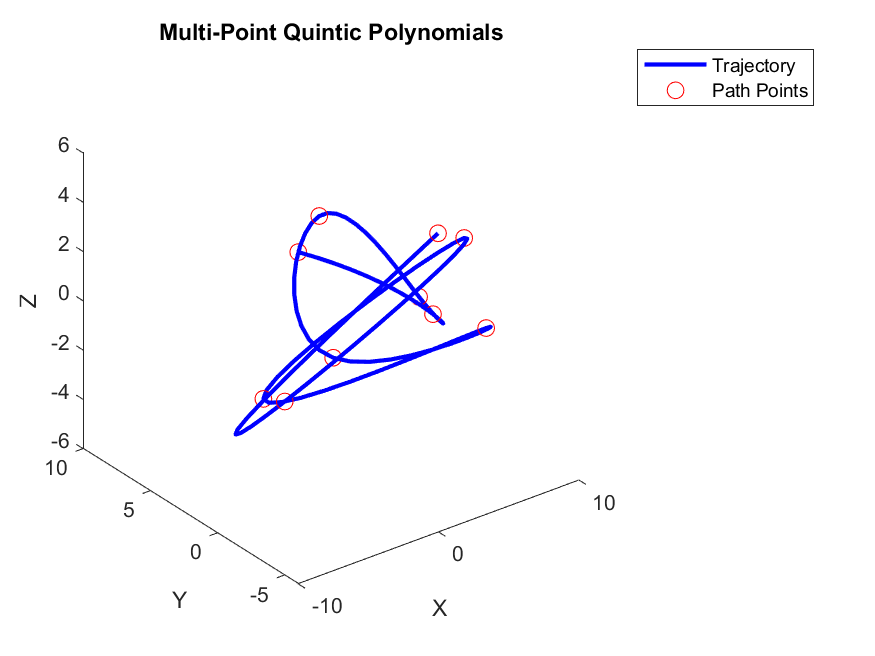
\includegraphics[width=0.4\textwidth]{figures/prob6/fig_9.png}
    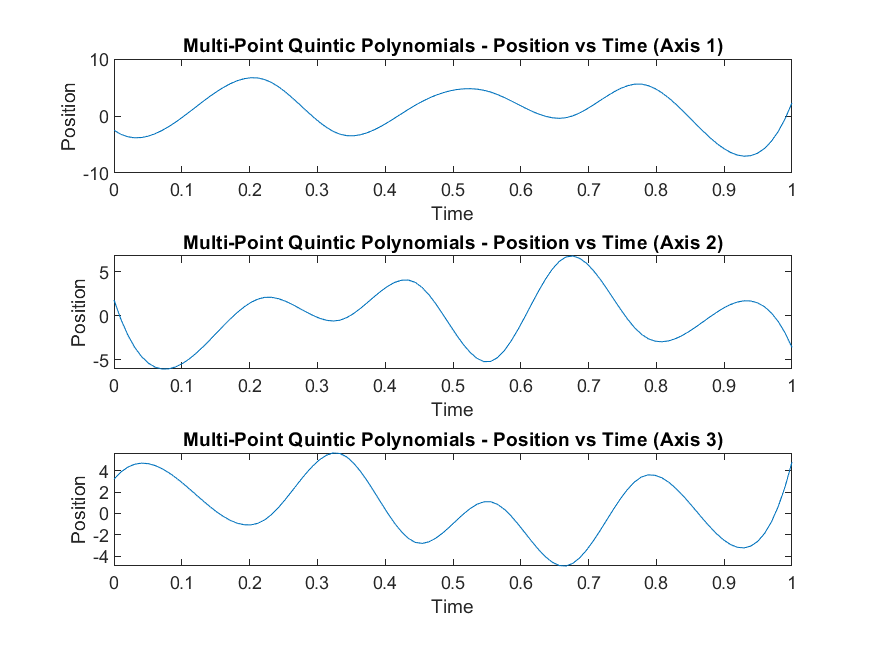
\includegraphics[width=0.4\textwidth]{figures/prob6/fig_10.png}
    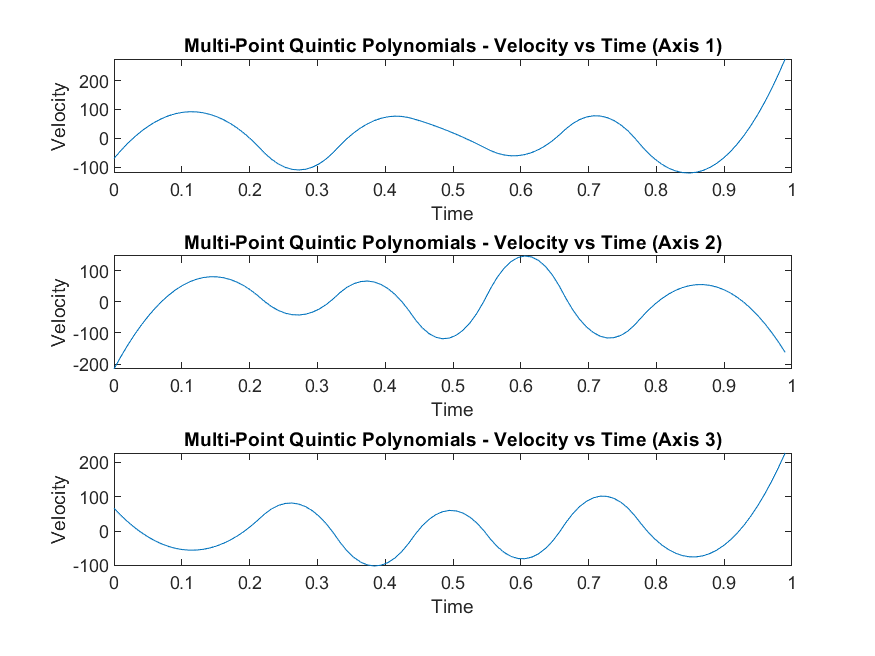
\includegraphics[width=0.4\textwidth]{figures/prob6/fig_11.png}
    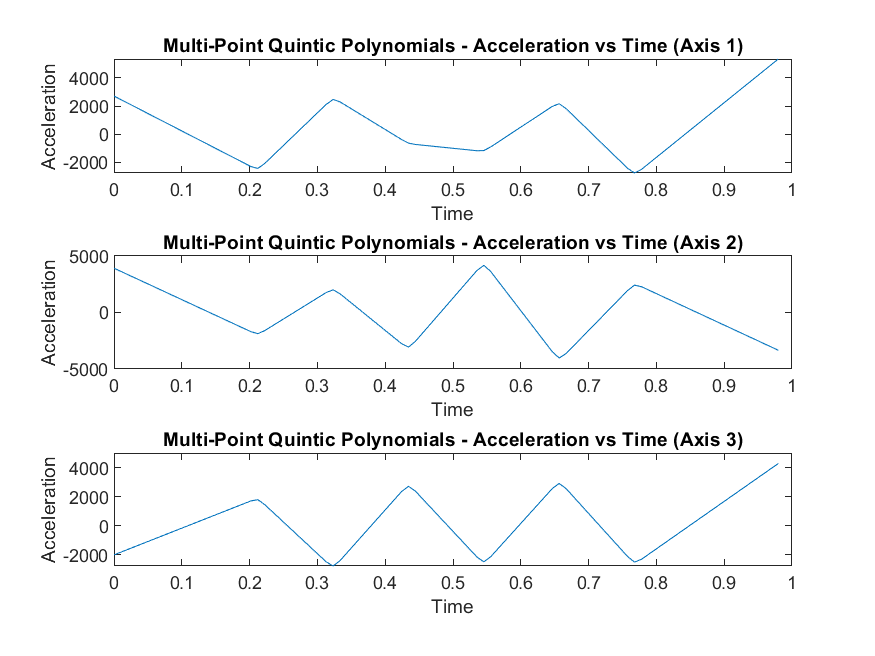
\includegraphics[width=0.4\textwidth]{figures/prob6/fig_12.png}
    \caption{Third four results for problem 6}
    \label{fig:res9}
\end{figure}

\begin{figure}[htbp]
    \centering
    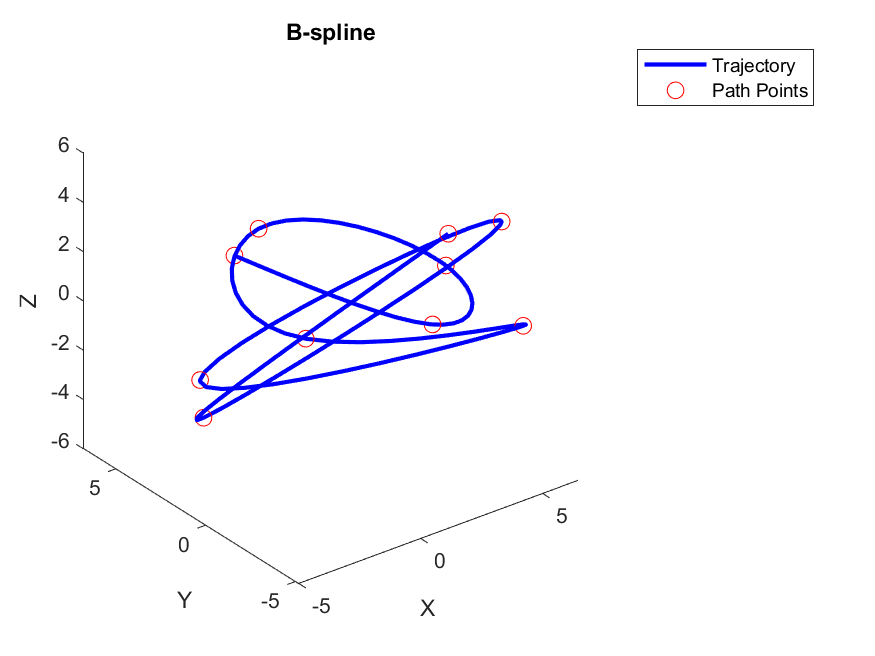
\includegraphics[width=0.4\textwidth]{figures/prob6/fig_13.png}
    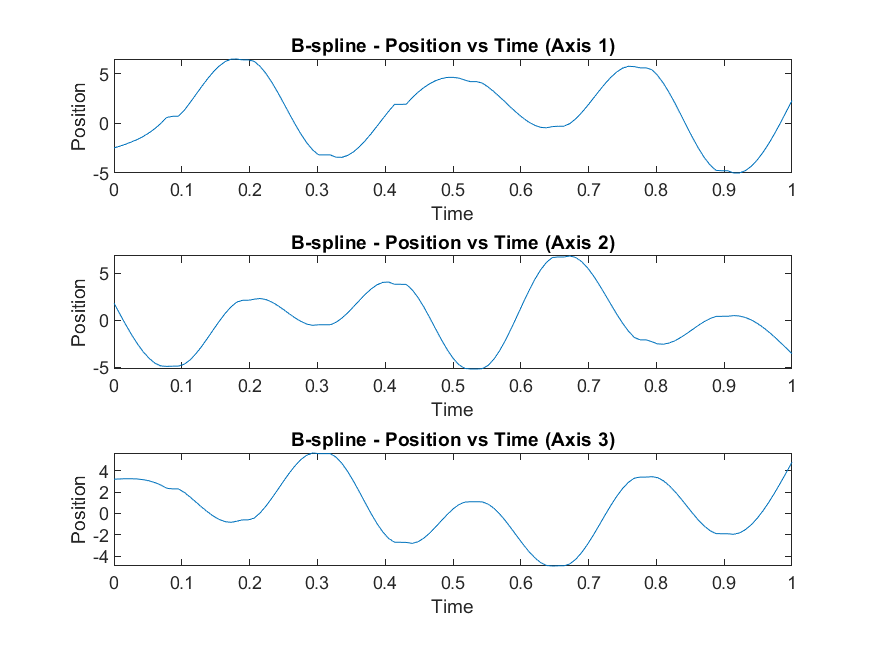
\includegraphics[width=0.4\textwidth]{figures/prob6/fig_14.png}
    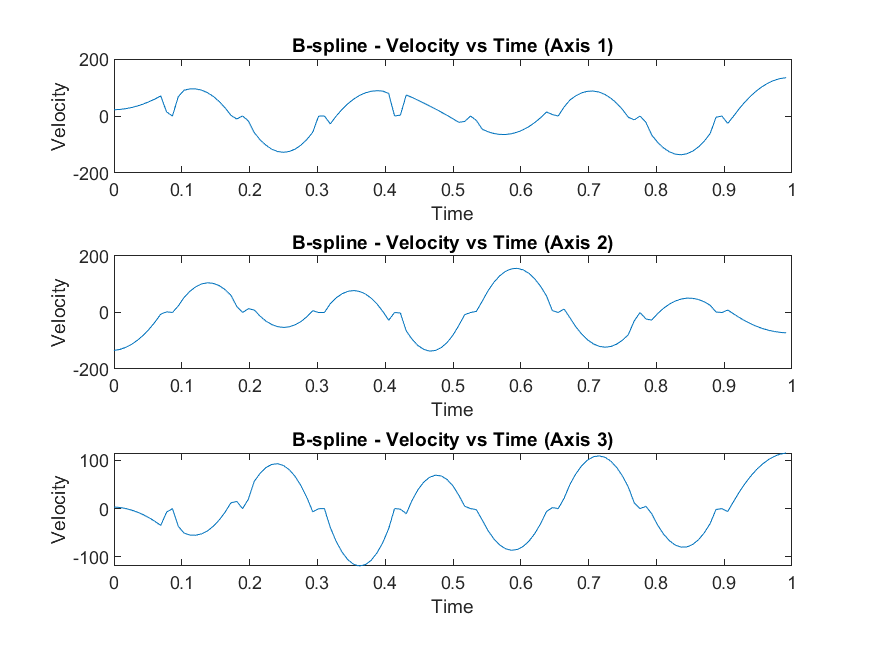
\includegraphics[width=0.4\textwidth]{figures/prob6/fig_15.png}
    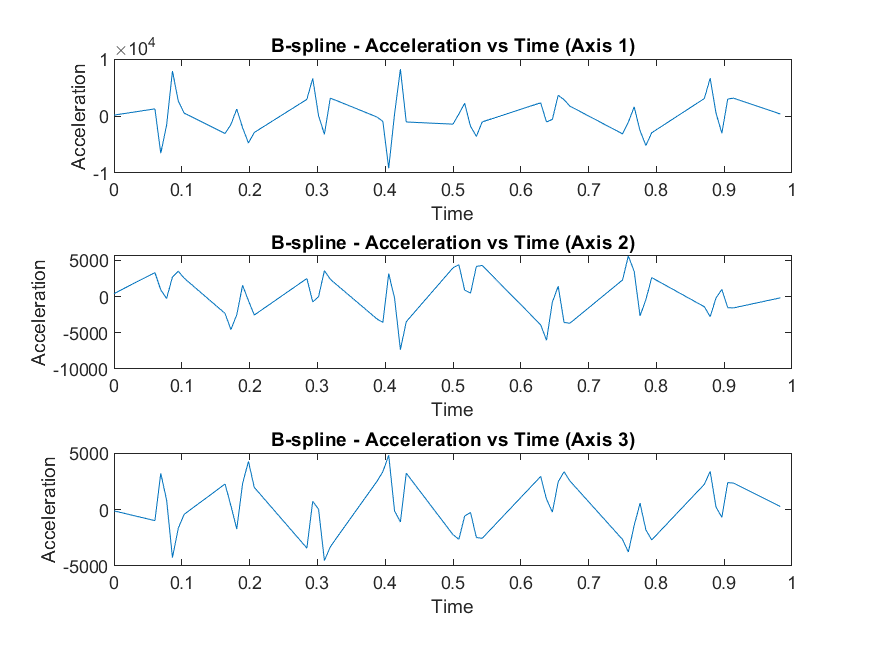
\includegraphics[width=0.4\textwidth]{figures/prob6/fig_16.png}
    \caption{Fourth four results for problem 6}
    \label{fig:res10}
\end{figure}

\end{document}
